\documentclass[11pt]{article}

\usepackage[margin=2.2cm]{geometry}
\usepackage{graphicx}
\usepackage{xcolor}
\usepackage{tikz}
\usetikzlibrary{shapes.geometric, arrows.meta, positioning, fit, calc}
\usepackage{booktabs}
\usepackage{tabularx}
\usepackage{longtable}
\usepackage{listings}
\usepackage{enumitem}
\usepackage{float}
\usepackage{caption}
\usepackage{amsmath}
\usepackage{hyperref}

\hypersetup{colorlinks=true, linkcolor=blue!50!black, urlcolor=blue!50!black, citecolor=blue!50!black}

\setcounter{tocdepth}{2}

\lstdefinestyle{py}{
    backgroundcolor=\color{gray!5},
    basicstyle=\ttfamily\footnotesize,
    breaklines=true,
    frame=single,
    rulecolor=\color{gray!40},
    numbers=left,
    numberstyle=\tiny\color{gray!60},
    keywordstyle=\color{blue!70!black}\bfseries,
    commentstyle=\color{green!35!black},
    stringstyle=\color{red!60!black},
    showstringspaces=false,
    language=Python,
    tabsize=4,
    columns=fullflexible,
}
\lstset{style=py}

\lstdefinestyle{sh}{
    backgroundcolor=\color{gray!5},
    basicstyle=\ttfamily\footnotesize,
    breaklines=true,
    frame=single,
    rulecolor=\color{gray!40},
    keywordstyle=\color{blue!70!black}\bfseries,
    commentstyle=\color{green!35!black},
    stringstyle=\color{red!60!black},
    showstringspaces=false,
    language=bash,
    columns=fullflexible,
}

\tikzset{
  startstop/.style={rectangle, rounded corners, minimum width=3.2cm, minimum height=0.9cm, text centered, draw=black, fill=green!15, font=\small},
  process/.style={rectangle, minimum width=3.6cm, minimum height=0.9cm, text centered, text width=3.4cm, draw=black, fill=blue!8, font=\small},
  decision/.style={diamond, aspect=2.4, minimum width=3cm, minimum height=0.9cm, text centered, text width=2.6cm, draw=black, fill=yellow!15, font=\small, inner sep=1pt},
  block/.style={rectangle, rounded corners, draw=black, align=center, font=\small, minimum height=1.1cm},
  arrowline/.style={-{Stealth}, thick},
}

\title{\textbf{Scene Graph Construction and Open-Vocabulary\\ Mobile Manipulation on the HSR-C Robot:\\ Methodology and Code Correlation}}
\author{HSR-C OVMM Project}
\date{\today}

\begin{document}

\maketitle

\begin{abstract}
This report documents how the project builds a 3D scene graph from a Gazebo
simulation (or from a real RGB-D scan), how an LLM is used to cluster
furniture into rooms and to reason about object locations, and how a single
mission command drives the HSR-C robot through navigation, active-perception
observation, open-vocabulary detection, and grasping. Every demo-day
requirement is mapped to the exact files and functions that implement it.
Particular attention is given to the scene-graph geometry pipeline: object
positions, sizes, and centroids are derived entirely from Gazebo's own model
description files (SDF collision geometry), with no hand-picked dimensions.
\end{abstract}

\tableofcontents
\newpage

\section{Introduction}

\subsection{Demo-Day Requirements}

The target capability set for the demo is:

\begin{enumerate}[label=(\arabic*)]
  \item From the ground truth of the Gazebo simulator, create a 3D scene graph programmatically.
  \item Use an LLM API to cluster furniture into rooms.
  \item For a given object to search for, support two scenarios:
        \textbf{Scenario A} -- the object is \emph{not} in the scene graph, so
        the LLM is queried for the object and predicts the top-$k$ candidate
        locations; \textbf{Scenario B} -- the object \emph{is} already in the
        scene graph, so its known location is used directly.
  \item The robot navigates to the first candidate location (either the
        LLM's top prediction, or the scene-graph location).
  \item The robot observes the location and either detects or does not detect
        the object.
  \item If detected: build an RGB-D point cloud of the object, plan a grasp,
        and move the arm.
  \item If not detected: move to the next predicted location; in Scenario B,
        once the known location fails, fall back to querying the LLM for
        predictions.
  \item Demonstrate active perception: control of the robot's head to look at
        candidate locations.
  \item Support the same scene-graph construction from a \emph{real} RGB-D
        scan, using Mask3D segmentation.
  \item Steps 3--7 must be runnable as a single command.
\end{enumerate}

\subsection{Scope of this document}

Section~\ref{sec:layout} gives a repository map. Section~\ref{sec:architecture}
shows the overall system architecture. Section~\ref{sec:scenegraph} is a deep
dive into the scene-graph construction pipeline, including the
\textbf{geometry-extraction module} that reads object dimensions and centroid
offsets directly from Gazebo's SDF model files (no hardcoded sizes anywhere).
Section~\ref{sec:correlation} walks through each demo-day requirement and
points to the exact code that implements it. Section~\ref{sec:missionflow}
gives detailed flowcharts of the single-command mission. Section~\ref{sec:run}
is a quick command reference.

\section{Repository Layout}
\label{sec:layout}

\begin{center}
\begin{tabularx}{\textwidth}{l X}
\toprule
\textbf{Path} & \textbf{Purpose} \\
\midrule
\texttt{core/perception/scene\_graph/} & \texttt{SceneGraph}, \texttt{ObjectNode}, the Gazebo and Mask3D scene-graph builders, and the new \texttt{gazebo\_geometry} module \\
\texttt{core/perception/segmentation/} & Mask3D output loader (\texttt{mask3d\_interface.py}) \\
\texttt{core/perception/detection/} & SAM3 REST client and mask$\to$pointcloud lifting \\
\texttt{core/perception/grasping/} & Geometric top-down grasp planner \\
\texttt{core/perception/} & \texttt{head\_geometry.py} -- pure pan/tilt geometry for active perception \\
\texttt{core/llm\_zone/} & DeepSeek-based room clustering, scene queries, and active-perception viewpoint geometry \\
\texttt{core/missions/} & \texttt{search\_and\_fetch.py} -- the ROS-agnostic mission runner (demo steps 3--7) \\
\texttt{ros2\_ws/src/fetcher/} & ROS 2 nodes: Nav2 goal execution, scene-graph builder entry point, \texttt{HsrRobotAdapter}, single-command mission node \\
\texttt{ros2\_ws/src/tmc\_gazebo/} & The \texttt{apartment.world.xacro} world file and all Gazebo model SDFs \\
\texttt{data/scene\_graph/} & Generated \texttt{graph.json}, \texttt{scene.json}, \texttt{rooms.json}, \texttt{objects/*.json} \\
\bottomrule
\end{tabularx}
\end{center}

\section{System Architecture}
\label{sec:architecture}

Figure~\ref{fig:architecture} shows the full pipeline. Two parallel inputs --
Gazebo's ground-truth world description, and a real RGB-D scan processed with
Mask3D -- are converted into the same \texttt{SceneGraph} / \texttt{ObjectNode}
representation and the same JSON files. From there, two DeepSeek-backed LLM
modules (room clustering and scene query) and the single-command mission
runner operate identically regardless of which pipeline produced the scene
graph.

\begin{figure}[H]
\centering
\resizebox{\textwidth}{!}{%
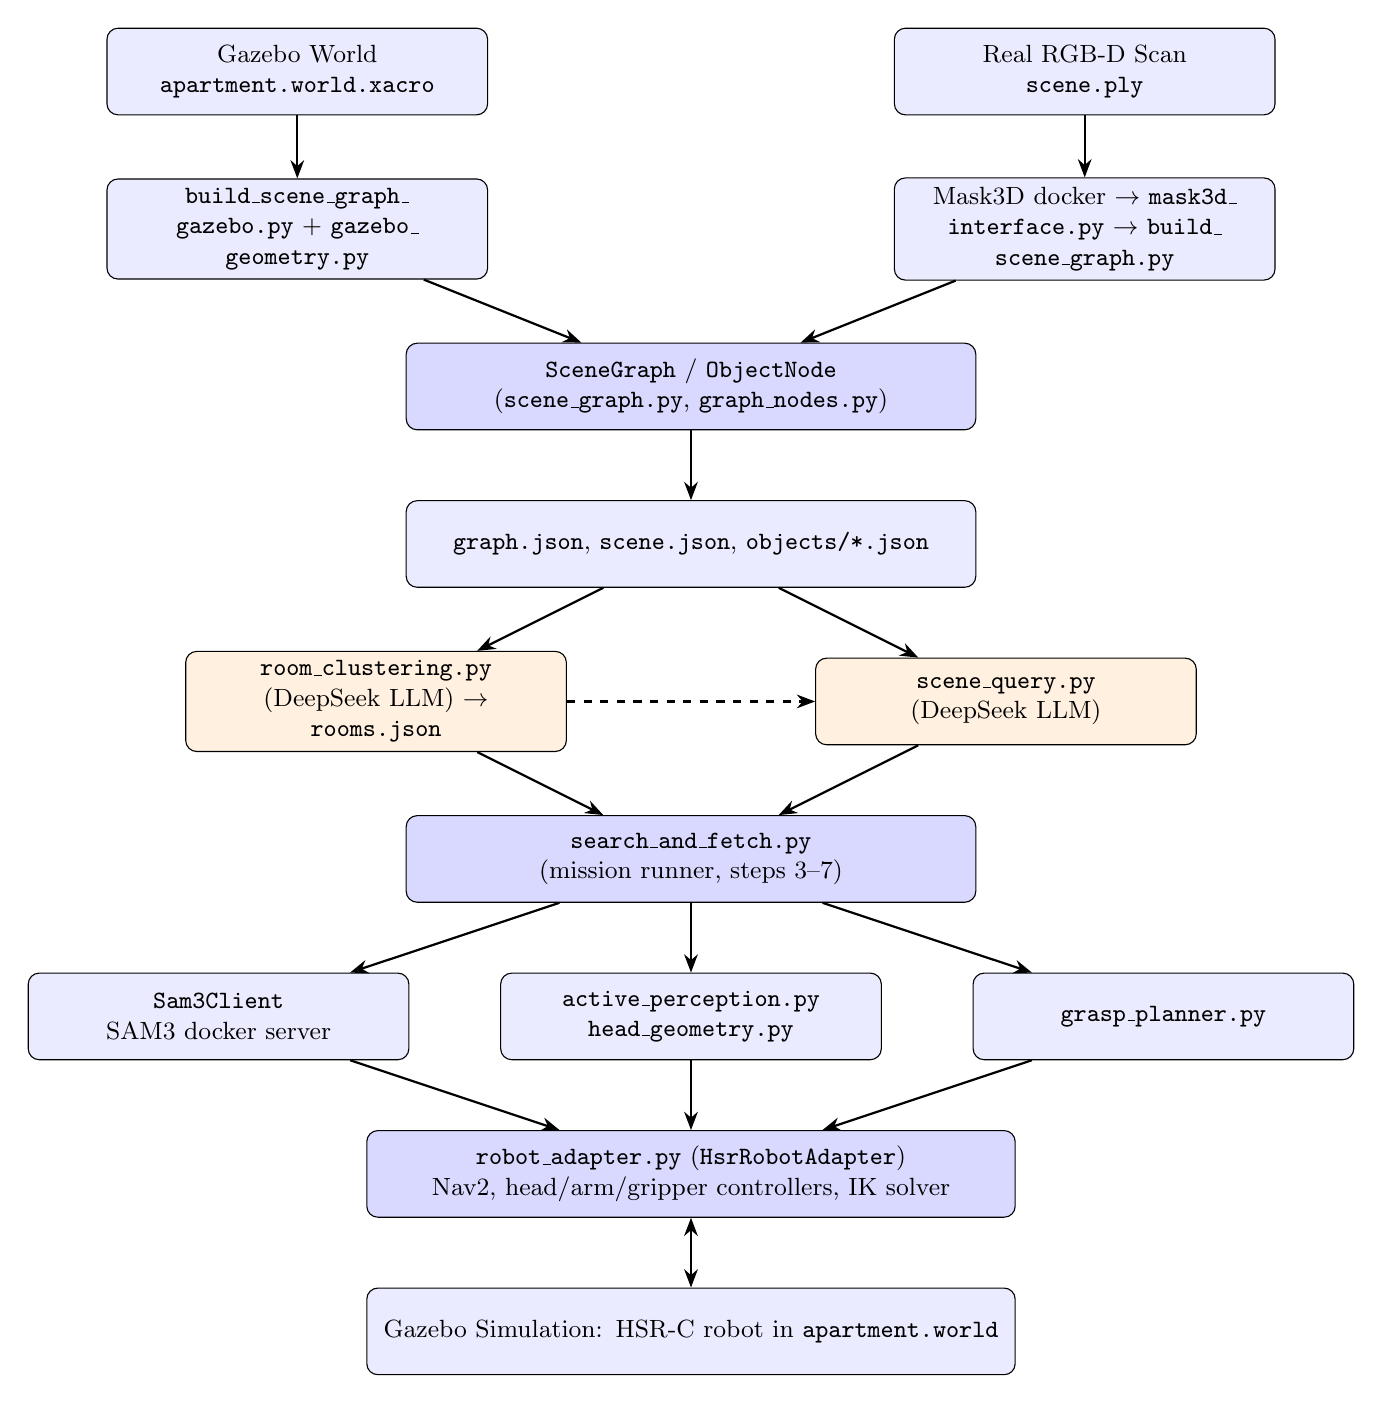
\begin{tikzpicture}
\node[block, fill=blue!8, text width=4.6cm] (gz) at (0,8) {Gazebo World\\\texttt{apartment.world.xacro}};
\node[block, fill=blue!8, text width=4.6cm] (scan) at (10,8) {Real RGB-D Scan\\\texttt{scene.ply}};

\node[block, fill=blue!8, text width=4.6cm] (gzbuild) at (0,6) {\texttt{build\_scene\_graph\_}\\\texttt{gazebo.py} + \texttt{gazebo\_}\\\texttt{geometry.py}};
\node[block, fill=blue!8, text width=4.6cm] (m3d) at (10,6) {Mask3D docker $\to$ \texttt{mask3d\_}\\\texttt{interface.py} $\to$ \texttt{build\_}\\\texttt{scene\_graph.py}};

\node[block, fill=blue!15, text width=7cm] (sg) at (5,4) {\texttt{SceneGraph} / \texttt{ObjectNode}\\(\texttt{scene\_graph.py}, \texttt{graph\_nodes.py})};

\node[block, fill=blue!8, text width=7cm] (json) at (5,2) {\texttt{graph.json}, \texttt{scene.json}, \texttt{objects/*.json}};

\node[block, fill=orange!12, text width=4.6cm] (rooms) at (1,0) {\texttt{room\_clustering.py}\\(DeepSeek LLM) $\to$\\ \texttt{rooms.json}};
\node[block, fill=orange!12, text width=4.6cm] (query) at (9,0) {\texttt{scene\_query.py}\\(DeepSeek LLM)};

\node[block, fill=blue!15, text width=7cm] (mission) at (5,-2) {\texttt{search\_and\_fetch.py}\\(mission runner, steps 3--7)};

\node[block, fill=blue!8, text width=4.6cm] (sam3) at (-1,-4) {\texttt{Sam3Client}\\SAM3 docker server};
\node[block, fill=blue!8, text width=4.6cm] (ap) at (5,-4) {\texttt{active\_perception.py}\\\texttt{head\_geometry.py}};
\node[block, fill=blue!8, text width=4.6cm] (grasp) at (11,-4) {\texttt{grasp\_planner.py}};

\node[block, fill=blue!15, text width=8cm] (adapter) at (5,-6) {\texttt{robot\_adapter.py} (\texttt{HsrRobotAdapter})\\Nav2, head/arm/gripper controllers, IK solver};

\node[block, fill=blue!8, text width=8cm] (sim) at (5,-8) {Gazebo Simulation: HSR-C robot in \texttt{apartment.world}};

\draw[arrowline] (gz) -- (gzbuild);
\draw[arrowline] (scan) -- (m3d);
\draw[arrowline] (gzbuild) -- (sg);
\draw[arrowline] (m3d) -- (sg);
\draw[arrowline] (sg) -- (json);
\draw[arrowline] (json) -- (rooms);
\draw[arrowline] (json) -- (query);
\draw[arrowline, dashed] (rooms) -- (query);
\draw[arrowline] (rooms) -- (mission);
\draw[arrowline] (query) -- (mission);
\draw[arrowline] (mission) -- (sam3);
\draw[arrowline] (mission) -- (ap);
\draw[arrowline] (mission) -- (grasp);
\draw[arrowline] (sam3) -- (adapter);
\draw[arrowline] (ap) -- (adapter);
\draw[arrowline] (grasp) -- (adapter);
\draw[{Stealth}-{Stealth}, thick] (adapter) -- (sim);
\end{tikzpicture}%
}
\caption{System architecture. Dashed arrow: room labels from
\texttt{rooms.json} enrich the LLM's location predictions in
\texttt{scene\_query.predict\_locations}. The double-headed arrow between the
robot adapter and Gazebo represents the bidirectional flow of commands
(Nav2 goals, joint trajectories) and sensor data (camera, depth, TF, joint
states).}
\label{fig:architecture}
\end{figure}

\section{Scene Graph Construction Methodology}
\label{sec:scenegraph}

This section explains, step by step, how
\path{core/perception/scene_graph/build_scene_graph_gazebo.py} turns
\path{apartment.world.xacro} into the \texttt{SceneGraph} object and its JSON
outputs -- and, in particular, how \textbf{every geometric quantity (object
position, size, centroid offset) is derived from Gazebo's own files}, with
no hand-picked numbers.

\subsection{World file parsing and the semantic registry}
\label{sec:worldparse}

\texttt{apartment.world.xacro} is a Xacro file: a templated XML format that
expands to plain SDF. \texttt{load\_registry()} shells out to the
\texttt{xacro} CLI and then walks the resulting \texttt{<world><include>}
elements:

\begin{lstlisting}[caption={\texttt{build\_scene\_graph\_gazebo.py}: world parsing (excerpt)}]
expanded = subprocess.run(
    ["xacro", str(world_xacro)], capture_output=True, text=True, check=True
).stdout
world = ET.fromstring(expanded).find("world")

registry = []
for include in world.findall("include"):
    name = include.findtext("name")
    label = NAME_TO_LABEL.get(name)
    if label is None:
        continue
    pose = tuple(float(v) for v in include.findtext("pose").split())
    dims, center = model_local_bbox(include.findtext("uri"))
    registry.append({"name": name, "label": label, "pose": pose,
                      "dims": dims, "center": center})
\end{lstlisting}

Each \texttt{<include>} in the expanded world file provides three pieces of
\textbf{ground truth}, read directly from the simulation description:

\begin{itemize}
  \item \texttt{<name>} -- the instance name (e.g.\ \texttt{chair00}), used only to look up a semantic label;
  \item \texttt{<uri>} -- a \texttt{model://<name>} reference to the object's SDF model, used to derive its geometry (Section~\ref{sec:geomextract});
  \item \texttt{<pose>x y z roll pitch yaw</pose>} -- the object's real pose in the world frame.
\end{itemize}

\paragraph{The only remaining hand-written table.} \texttt{NAME\_TO\_LABEL}
maps each \texttt{<include><name>} to a human-readable semantic category
(Table~\ref{tab:nametolabel}). This is \emph{semantic} configuration -- it
tells the system ``\texttt{chair00} is a chair'' -- exactly analogous to the
ScanNet200 label table (\path{core/utils/scannet_200_labels.py}) used by the
real-scan pipeline, or the \texttt{IMMOVABLE\_LABELS} list in
\path{build_scene_graph.py}. It contains \emph{no} sizes, positions, or
offsets. \texttt{IMMOVABLE\_LABELS\_GZ} similarly lists which categories count
as furniture (movable objects connect to the nearest one of these).
\texttt{<include>} names not present in \texttt{NAME\_TO\_LABEL} -- walls,
doors, door stoppers, the lawn/garden mesh, etc. -- are structural and
skipped.

\begin{center}
\begin{longtable}{l l l c}
\toprule
\textbf{\texttt{<include><name>}} & \textbf{\texttt{model://} URI} & \textbf{Label} & \textbf{Kind} \\
\midrule
\endhead
\texttt{wagon} & \texttt{wagon} & trolley & furniture \\
\texttt{nasal\_cupsul} & \texttt{nasal\_inflammation\_capsul} & medicine box & object \\
\texttt{sofa01}, \texttt{sofa02} & \texttt{sofa-fix} & couch & furniture \\
\texttt{kitchen\_lowtable} & \texttt{kitchen\_lowtable} & coffee table & furniture \\
\texttt{office\_desk01/02/06} & \texttt{office\_desk} & desk & furniture \\
\texttt{chair00/01/02/05} & \texttt{kitchen\_chair} & chair & furniture \\
\texttt{living\_sideboard} & \texttt{openable\_living\_sideboard} & cabinet & furniture \\
\texttt{wallet} & \texttt{wallet} & wallet & object \\
\texttt{high\_table01} & \texttt{high\_table} & table & furniture \\
\texttt{high\_shelf01/02/03} & \texttt{high\_shelf} & shelf & furniture \\
\texttt{hsr\_orange\_02} & \texttt{hsr\_orange} & orange & object \\
\texttt{hsr\_pringles\_01/02} & \texttt{hsr\_pringles} & pringles can & object \\
\texttt{apple\_01} & \texttt{apple} & apple & object \\
\texttt{banana\_01} & \texttt{banana} & banana & object \\
\texttt{pear\_01} & \texttt{pear} & pear & object \\
\bottomrule
\caption{\texttt{NAME\_TO\_LABEL} registry: 24 \texttt{<include>} instances,
15 unique \texttt{model://} URIs. ``Kind'' is determined by membership in
\texttt{IMMOVABLE\_LABELS\_GZ}.}
\label{tab:nametolabel}
\end{longtable}
\end{center}

\subsection{Geometry extraction from Gazebo SDF}
\label{sec:geomextract}

\subsubsection{Motivation}

An earlier version of this builder paired each label with a hand-picked
\texttt{(width, depth, height, center\_z)} tuple (a module-level
\texttt{LABEL\_GEOMETRY} dictionary). Those numbers were rough guesses and
were shared across every instance of a label, so e.g.\ all four kitchen
chairs used the same guessed size regardless of the model actually placed in
the world. \path{core/perception/scene_graph/gazebo_geometry.py} replaces
this entirely: it loads each model's own SDF file and computes its bounding
box from the \textbf{collision geometry} Gazebo itself uses for physics --
the same shapes the simulator would use to detect the robot bumping into the
object.

\subsubsection{SDF frame hierarchy and pose composition}

A Gazebo \texttt{model://} reference resolves to a directory containing
\texttt{model.config} (which names the actual \texttt{.sdf} file) and that
SDF file's \texttt{<model>} element, which contains one or more
\texttt{<link>} elements, each containing one or more \texttt{<collision>}
(or \texttt{<visual>}) elements, each with a \texttt{<geometry>}. Every level
may carry its own \texttt{<pose>x y z roll pitch yaw</pose>}, defaulting to
identity if absent. Figure~\ref{fig:framehierarchy} shows how these poses
compose to bring a shape's local geometry into the model frame, and how the
world-file \texttt{<include><pose>} (Section~\ref{sec:worldparse}) then
brings the model frame into the world frame.

\begin{figure}[H]
\centering
\begin{tikzpicture}[node distance=1.6cm]
\node[block, fill=blue!8, text width=6.5cm] (world) {World frame (\path{apartment.world})};
\node[block, fill=blue!8, text width=6.5cm, below=of world] (model) {Model frame\\\textit{applied by} \path{build_scene_graph_gazebo.py} \textit{using} \texttt{<include><pose>}};
\node[block, fill=blue!8, text width=6.5cm, below=of model] (link) {Link frame\\\textit{applied by} \texttt{gazebo\_geometry} \textit{using} \texttt{<model><pose>} $\times$ \texttt{<link><pose>}};
\node[block, fill=blue!8, text width=6.5cm, below=of link] (shape) {Collision/Visual frame\\\textit{applied by} \texttt{gazebo\_geometry} \textit{using} \texttt{<collision><pose>}};
\node[block, fill=blue!15, text width=6.5cm, below=of shape] (geom) {Geometry-local frame: 8 AABB corners of \texttt{<box>}/\texttt{<cylinder>}/\texttt{<sphere>}/\texttt{<mesh>}};

\draw[arrowline] (world) -- (model) node[midway, right, font=\scriptsize] {$T_{\text{include}}$};
\draw[arrowline] (model) -- (link) node[midway, right, font=\scriptsize] {$T_{\text{model}} \cdot T_{\text{link}}$};
\draw[arrowline] (link) -- (shape) node[midway, right, font=\scriptsize] {$T_{\text{collision}}$};
\draw[arrowline] (shape) -- (geom) node[midway, right, font=\scriptsize] {shape-local corners};
\end{tikzpicture}
\caption{Pose composition chain. Every $T$ is built by
\texttt{pose\_to\_matrix()} from an SDF \texttt{<pose>x y z roll pitch
yaw</pose>} string (identity if the element is absent). The bottom three
levels (model, link, collision) are composed by
\texttt{gazebo\_geometry.model\_local\_bbox()} to give a single bounding box
in the \emph{model} frame; \texttt{build\_scene\_graph\_gazebo.py} then applies
$T_{\text{include}}$ (the world-file pose) when sampling points
(Section~\ref{sec:synth}).}
\label{fig:framehierarchy}
\end{figure}

All rotations use the SDF convention $R = R_z(\text{yaw}) \cdot
R_y(\text{pitch}) \cdot R_x(\text{roll})$ and $p_{\text{world}} = R \, p_{\text{local}} + t$,
implemented once and shared by both the geometry module and the point
synthesizer:

\begin{lstlisting}[caption={\texttt{gazebo\_geometry.py}: shared rotation and pose-matrix helpers}]
def euler_to_matrix(roll, pitch, yaw):
    cr, sr = np.cos(roll), np.sin(roll)
    cp, sp = np.cos(pitch), np.sin(pitch)
    cy, sy = np.cos(yaw), np.sin(yaw)
    Rx = np.array([[1, 0, 0], [0, cr, -sr], [0, sr, cr]])
    Ry = np.array([[cp, 0, sp], [0, 1, 0], [-sp, 0, cp]])
    Rz = np.array([[cy, -sy, 0], [sy, cy, 0], [0, 0, 1]])
    return Rz @ Ry @ Rx

def pose_to_matrix(pose_text):
    T = np.eye(4)
    if pose_text is None:
        return T                      # default pose = identity
    x, y, z, roll, pitch, yaw = (float(v) for v in pose_text.split())
    T[:3, :3] = euler_to_matrix(roll, pitch, yaw)
    T[:3, 3] = [x, y, z]
    return T
\end{lstlisting}

\subsubsection{Resolving \texttt{model://} URIs}

\texttt{GAZEBO\_MODEL\_PATH} (set by the ROS 2 workspace setup scripts) lists
directories containing model packages. \texttt{resolve\_uri()} searches it
for a directory matching the URI's model name, and \texttt{\_model\_sdf\_path()}
reads that model's \texttt{model.config} to find the actual \texttt{.sdf}
filename (SDF format versions are mapped to filenames there, e.g.\
\texttt{model-1\_4.sdf}):

\begin{lstlisting}[caption={\texttt{gazebo\_geometry.py}: URI resolution (excerpt)}]
def resolve_uri(uri):
    if not uri.startswith("model://"):
        return Path(uri)
    name, _, sub = uri[len("model://"):].partition("/")
    for base in _gazebo_model_paths():        # GAZEBO_MODEL_PATH entries
        candidate = base / name
        if candidate.is_dir():
            return candidate / sub if sub else candidate
    raise FileNotFoundError(f"Could not resolve '{uri}' via GAZEBO_MODEL_PATH")

def _model_sdf_path(model_dir):
    config = ET.parse(model_dir / "model.config").getroot()
    return model_dir / config.findtext("sdf")
\end{lstlisting}

\subsubsection{Collision shape primitives}

For each \texttt{<collision>} (falling back to \texttt{<visual>} if a link has
none), \texttt{\_shape\_corners()} dispatches on the geometry type and returns
the 8 corners of that shape's axis-aligned bounding box in its \emph{own}
local frame:

\begin{itemize}
  \item \textbf{box} -- \texttt{<size>w d h</size>} $\to$ corners at $(\pm w/2, \pm d/2, \pm h/2)$.
  \item \textbf{cylinder} -- \texttt{<radius>}, \texttt{<length>} (axis along local $Z$, per SDF convention) $\to$ corners of a $(\pm r, \pm r, \pm \text{length}/2)$ box.
  \item \textbf{sphere} -- \texttt{<radius>} $\to$ corners of a $(\pm r, \pm r, \pm r)$ cube (a safe enclosing box for a sphere).
  \item \textbf{mesh} -- see below.
\end{itemize}

\begin{lstlisting}[caption={\texttt{gazebo\_geometry.py}: primitive corner helpers}]
_CORNER_SIGNS = np.array(list(itertools.product([-1, 1], repeat=3)))

def _box_corners(size_text):
    half_extent = np.array([float(v) for v in size_text.split()]) / 2.0
    return _CORNER_SIGNS * half_extent

def _cylinder_corners(geom):
    r = float(geom.findtext("radius"))
    length = float(geom.findtext("length"))
    return _CORNER_SIGNS * np.array([r, r, length / 2.0])

def _sphere_corners(geom):
    r = float(geom.findtext("radius"))
    return _CORNER_SIGNS * r
\end{lstlisting}

\subsubsection{Mesh shapes and the COLLADA unit pitfall}
\label{sec:colladaunit}

Several models (the sofa, kitchen chairs, the table legs, the wallet, the
banana) use a \texttt{<mesh><uri>...\,.dae\,/\,.stl</uri></mesh>} collision
shape instead of a primitive. These are loaded with \texttt{trimesh} and their
axis-aligned bounds are used directly. There is one important subtlety:
\textbf{COLLADA (\texttt{.dae}) files declare their own unit of length} in an
\texttt{<asset><unit meter="X" .../></asset>} tag, and \texttt{trimesh} does
\emph{not} apply this automatically.

While building this module, \path{sofa-fix/meshes/sofa_seat.dae} was found to
declare \texttt{<unit meter="0.1" name="decimeter"/>}. Loading it naively gave
an absurd $7.76\,\text{m} \times 12.57\,\text{m} \times 4.76\,\text{m}$
bounding box for a sofa seat. \texttt{\_collada\_unit\_meters()} parses this
tag directly from the XML (defaulting to $1.0$ if absent) and the loaded mesh
is scaled by it before computing bounds -- after which the sofa seat mesh
correctly measures $0.776\,\text{m} \times 1.257\,\text{m} \times
0.476\,\text{m}$:

\begin{lstlisting}[caption={\texttt{gazebo\_geometry.py}: mesh bounds with COLLADA unit correction}]
COLLADA_NS = {"c": "http://www.collada.org/2005/11/COLLADASchema"}

def _collada_unit_meters(dae_path):
    unit = ET.parse(dae_path).getroot().find(".//c:asset/c:unit", COLLADA_NS)
    return float(unit.get("meter", "1.0")) if unit is not None else 1.0

@lru_cache(maxsize=None)
def _mesh_local_bounds(mesh_path):
    path = Path(mesh_path)
    mesh = trimesh.load(str(path), force="mesh")
    if path.suffix.lower() == ".dae":
        mesh.apply_scale(_collada_unit_meters(path))
    return mesh.bounds[0].copy(), mesh.bounds[1].copy()

def _mesh_corners(geom):
    path = resolve_uri(geom.findtext("uri"))
    scale = np.array([float(v) for v in (geom.findtext("scale") or "1 1 1").split()])
    bmin, bmax = _mesh_local_bounds(str(path))
    bmin, bmax = bmin * scale, bmax * scale
    return np.array(list(itertools.product(*zip(bmin, bmax))))
\end{lstlisting}

After the unit correction, the SDF's own \texttt{<scale sx sy sz>} (default
$1,1,1$) is applied on top -- this is the scale Gazebo itself applies when
instantiating the mesh as a collision shape, so the two corrections are
independent and both necessary.

\subsubsection{Assembling a model's bounding box}
\label{sec:modelbbox}

\texttt{model\_local\_bbox(uri)} is the single entry point used by the scene
graph builder. For every \texttt{<link>} and every
\texttt{<collision>}/\texttt{<visual>} shape inside it, the shape's local
corners are transformed through $T_{\text{collision}}$, then $T_{\text{link}}$,
then $T_{\text{model}}$ (Figure~\ref{fig:framehierarchy}); all resulting
corners across the whole model are pooled, and the union's axis-aligned
bounding box gives \texttt{dims} (extent) and \texttt{center} (offset of the
box's centre from the model origin):

\begin{lstlisting}[caption={\texttt{gazebo\_geometry.py}: \texttt{model\_local\_bbox} -- the core algorithm}]
@lru_cache(maxsize=None)
def model_local_bbox(model_uri):
    model_dir = resolve_uri(model_uri)
    model = ET.parse(_model_sdf_path(model_dir)).getroot().find("model")
    model_pose = pose_to_matrix(model.findtext("pose"))

    corners = []
    for link in model.findall("link"):
        link_pose = model_pose @ pose_to_matrix(link.findtext("pose"))
        for shape in link.findall("collision") or link.findall("visual"):
            local_corners = _shape_corners(shape.find("geometry"))
            if local_corners is None:
                continue
            shape_pose = link_pose @ pose_to_matrix(shape.findtext("pose"))
            corners.append(local_corners @ shape_pose[:3, :3].T + shape_pose[:3, 3])

    points = np.concatenate(corners, axis=0)
    bbox_min, bbox_max = points.min(axis=0), points.max(axis=0)
    return bbox_max - bbox_min, (bbox_min + bbox_max) / 2.0
\end{lstlisting}

The \texttt{@lru\_cache} means each unique \texttt{model://} URI is parsed
(and any meshes loaded) exactly once, no matter how many \texttt{<include>}s
reference it -- e.g.\ the four \texttt{kitchen\_chair} instances, three
\texttt{high\_shelf} instances, three \texttt{office\_desk} instances, and two
\texttt{sofa-fix} / \texttt{hsr\_pringles} instances each share one
computation. Figure~\ref{fig:geomflow} shows this as a flowchart.

\begin{figure}[H]
\centering
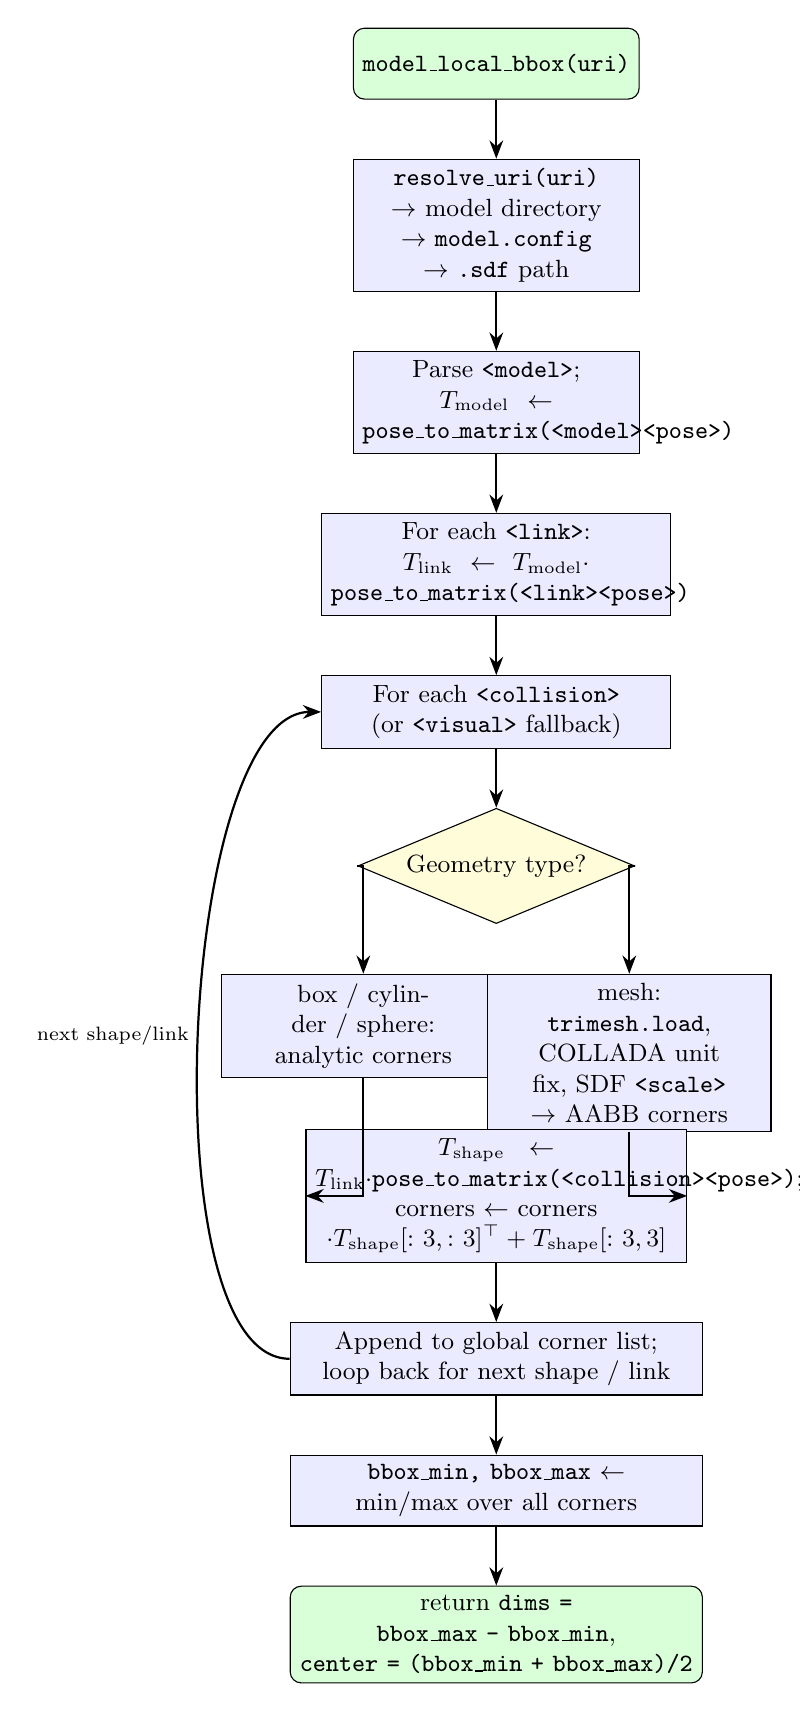
\begin{tikzpicture}[node distance=0.75cm and 1.2cm]
\node[startstop] (start) {\texttt{model\_local\_bbox(uri)}};
\node[process, below=of start] (resolve) {\texttt{resolve\_uri(uri)} $\to$ model directory $\to$ \texttt{model.config} $\to$ \texttt{.sdf} path};
\node[process, below=of resolve] (parse) {Parse \texttt{<model>}; $T_{\text{model}} \gets$ \texttt{pose\_to\_matrix(<model><pose>)}};
\node[process, below=of parse, text width=4.2cm] (link) {For each \texttt{<link>}:\\ $T_{\text{link}} \gets T_{\text{model}} \cdot$ \texttt{pose\_to\_matrix(<link><pose>)}};
\node[process, below=of link, text width=4.2cm] (shapeloop) {For each \texttt{<collision>} (or \texttt{<visual>} fallback)};
\node[decision, below=of shapeloop] (type) {Geometry type?};
\node[process, below left=1.0cm and -1.0cm of type, text width=2.6cm] (prim) {box / cylinder / sphere: analytic corners};
\node[process, below right=1.0cm and -1.0cm of type, text width=2.6cm] (mesh) {mesh: \texttt{trimesh.load}, COLLADA unit fix, SDF \texttt{<scale>} $\to$ AABB corners};
\node[process, below=2.6cm of type, text width=4.6cm] (transform) {$T_{\text{shape}} \gets T_{\text{link}} \cdot$\texttt{pose\_to\_matrix(<collision><pose>)};\\ corners $\gets$ corners $\cdot T_{\text{shape}}[:3,:3]^\top + T_{\text{shape}}[:3,3]$};
\node[process, below=of transform, text width=5cm] (accum) {Append to global corner list; loop back for next shape / link};
\node[process, below=of accum, text width=5cm] (bbox) {\texttt{bbox\_min, bbox\_max} $\gets$ min/max over all corners};
\node[startstop, below=of bbox, text width=5cm] (ret) {return \texttt{dims = bbox\_max - bbox\_min},\\ \texttt{center = (bbox\_min + bbox\_max)/2}};

\draw[arrowline] (start) -- (resolve);
\draw[arrowline] (resolve) -- (parse);
\draw[arrowline] (parse) -- (link);
\draw[arrowline] (link) -- (shapeloop);
\draw[arrowline] (shapeloop) -- (type);
\draw[arrowline] (type) -| (prim);
\draw[arrowline] (type) -| (mesh);
\draw[arrowline] (prim) |- (transform);
\draw[arrowline] (mesh) |- (transform);
\draw[arrowline] (transform) -- (accum);
\draw[arrowline] (accum.west) .. controls +(left:1.8cm) and +(left:1.8cm) .. (shapeloop.west) node[midway, left, font=\scriptsize] {next shape/link};
\draw[arrowline] (accum) -- (bbox);
\draw[arrowline] (bbox) -- (ret);
\end{tikzpicture}
\caption{\texttt{gazebo\_geometry.model\_local\_bbox()}: from a
\texttt{model://} URI to a local-frame bounding box (\texttt{dims},
\texttt{center}), used by every \texttt{<include>} referencing that model.}
\label{fig:geomflow}
\end{figure}

\subsection{Point cloud synthesis}
\label{sec:synth}

Back in \path{build_scene_graph_gazebo.py}, \texttt{synthesize\_points()}
takes the \texttt{(dims, center)} pair from \texttt{model\_local\_bbox} and the
\texttt{<include><pose>} from the world file, and produces a small
$5\times5\times5$ grid of points filling that box, rotated and translated into
the world frame -- exactly the kind of point set the Mask3D pipeline would
hand to \texttt{SceneGraph.add\_node()} for a real scan:

\begin{lstlisting}[caption={\texttt{build\_scene\_graph\_gazebo.py}: \texttt{synthesize\_points}}]
def synthesize_points(pose, dims, center, n=5):
    x, y, z, roll, pitch, yaw = pose
    w, d, h = dims
    cx, cy, cz = center

    xs = cx + np.linspace(-w / 2, w / 2, n)
    ys = cy + np.linspace(-d / 2, d / 2, n)
    zs = cz + np.linspace(-h / 2, h / 2, n)
    grid = np.stack(np.meshgrid(xs, ys, zs, indexing="ij"), axis=-1).reshape(-1, 3)

    R = euler_to_matrix(roll, pitch, yaw)
    return grid @ R.T + np.array([x, y, z])
\end{lstlisting}

\subsection{ObjectNode: centroid, pose, and dimensions}
\label{sec:objectnode}

Whether points come from \texttt{synthesize\_points} (Gazebo) or from a Mask3D
instance mask (real scan), they are handed to
\path{core/perception/scene_graph/graph_nodes.py}'s \texttt{ObjectNode}, which
computes everything the rest of the system needs:

\begin{lstlisting}[caption={\texttt{graph\_nodes.py}: centroid, PCA pose, and minimal OBB dimensions}]
def __init__(self, object_id, color, sem_label, points, mesh_mask, confidence=None, movable=True):
    ...
    self.centroid = np.mean(points, axis=0)
    ...
    self.update_hull_tree()
    self.compute_pose(self.points, self.centroid)
    self.get_dimensions()

def compute_pose(self, points, centroid):
    points_centered = points - centroid
    covariance_matrix = np.cov(points_centered, rowvar=False)
    eigenvalues, eigenvectors = np.linalg.eigh(covariance_matrix)
    sorted_idx = np.argsort(eigenvalues)[::-1]
    eigenvectors = eigenvectors[:, sorted_idx]
    R = eigenvectors
    if np.linalg.det(R) < 0:
        R[:, -1] *= -1
    object_pose = np.eye(4)
    object_pose[:3, :3] = R
    object_pose[:3, 3] = centroid
    self.pose = object_pose

def get_dimensions(self):
    point_cloud = o3d.geometry.PointCloud()
    point_cloud.points = o3d.utility.Vector3dVector(self.points)
    obb = point_cloud.get_minimal_oriented_bounding_box()
    height_idx = np.argmax(np.abs(obb.R.T @ [0, 0, 1]))
    width_depth = sorted([i for i in range(3) if i != height_idx],
                          key=lambda i: obb.extent[i], reverse=True)
    order = width_depth + [height_idx]
    self.bb = obb
    self.dimensions = obb.extent[order]
\end{lstlisting}

Two consequences are worth noting for interpreting the output table
(Table~\ref{tab:results}):

\begin{itemize}
  \item \textbf{Centroid} is the mean of the synthesized grid, i.e.\
        $\text{pose}_{xyz} + R(\text{roll,pitch,yaw}) \cdot \text{center}$ --
        the real world-frame position of the geometric centre of the
        object's collision geometry.
  \item \textbf{Dimensions} come from Open3D's \emph{minimal oriented bounding
        box} of the (rotated) point grid, then reordered so the axis most
        aligned with world $Z$ is reported last. For an object rotated by
        $90^\circ$ about $Z$ (e.g.\ a desk with \texttt{yaw=-1.5708}), the
        reported width and depth are swapped relative to the model's own
        $(w,d,h)$ -- this is expected and is the same convention
        \path{build_scene_graph.py} uses for real Mask3D instances.
\end{itemize}

\subsection{SceneGraph: connections and persistence}
\label{sec:scenegraphclass}

\path{core/perception/scene_graph/scene_graph.py}'s \texttt{SceneGraph} class
is shared, unchanged, by both builders. \texttt{add\_node()} marks a node
immovable if its label is in the builder's \texttt{immovable} list;
\texttt{update\_connection()} gives every \emph{movable} node one outgoing
edge to its nearest \emph{immovable} node (by centroid distance) -- e.g.\ the
apple connects to the high shelf it sits on:

\begin{lstlisting}[caption={\texttt{scene\_graph.py}: \texttt{add\_node} and \texttt{update\_connection}}]
def add_node(self, color, sem_label, points, mesh_mask, confidence, movable=True):
    if self.label_mapping.get(sem_label, "ID not found") in self.immovable:
        self.nodes[self.index] = ObjectNode(self.index, np.array([0.5,0.5,0.5]),
                                             sem_label, points, mesh_mask, confidence, movable=False)
    else:
        self.nodes[self.index] = ObjectNode(self.index, color, sem_label,
                                             points, mesh_mask, confidence, movable=movable)
    self.labels.setdefault(sem_label, []).append(self.index)
    self.ids.append(self.index)
    self.index += 1

def update_connection(self, node):
    min_index, min_dist = None, None
    if node.movable:
        for other in self.nodes.values():
            if not other.movable:
                dist = np.linalg.norm(node.centroid - other.centroid)
                if min_dist is None or dist < min_dist:
                    min_dist, min_index = dist, other.object_id
    ...  # record one outgoing edge node -> min_index
\end{lstlisting}

After all nodes are added, \texttt{build\_from\_world()} (Gazebo) /
\texttt{build\_from\_mask3d()} (real scan) both call \texttt{update\_connection}
for every node, rebuild a \texttt{scipy.spatial.KDTree} over centroids, assign
colours via \texttt{color\_with\_ibm\_palette()}, and call
\texttt{scene\_graph.save\_all(graph\_dir)}, which writes:

\begin{itemize}
  \item \texttt{graph.json} -- node ids/labels, the \texttt{connections} map (movable id $\to$ furniture id), and the list of immovable ids/labels;
  \item \texttt{scene.json} -- \texttt{\{furniture\_id: \{label, centroid, dimensions\}\}} for every immovable node;
  \item \texttt{objects/\{id\}.json} -- one file per movable object with id, label, centroid, dimensions, PCA pose, and confidence.
\end{itemize}

\subsection{End-to-end build flow}

Figure~\ref{fig:buildflow} ties Sections~\ref{sec:worldparse}--\ref{sec:scenegraphclass}
together as the top-level flow of
\path{build_scene_graph_gazebo.py}'s \texttt{main()} /
\texttt{build\_from\_world()}.

\begin{figure}[H]
\centering
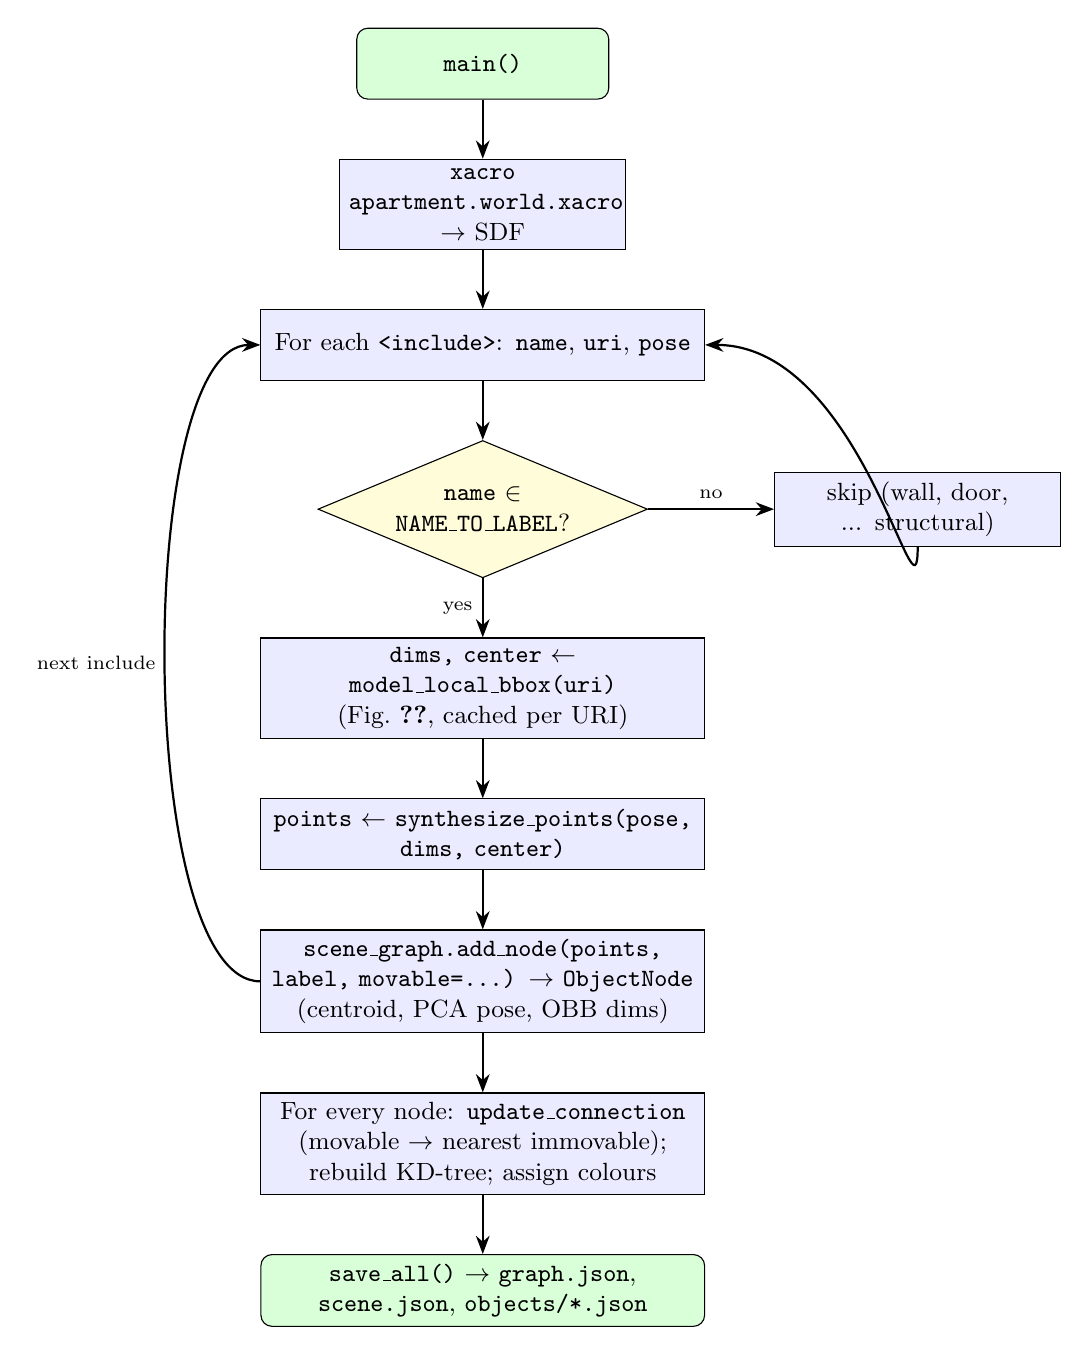
\begin{tikzpicture}[node distance=0.75cm]
\node[startstop] (start) {\texttt{main()}};
\node[process, below=of start] (xacro) {\texttt{xacro apartment.world.xacro} $\to$ SDF};
\node[process, below=of xacro, text width=5.4cm] (includes) {For each \texttt{<include>}: \texttt{name}, \texttt{uri}, \texttt{pose}};
\node[decision, below=of includes] (known) {\texttt{name} $\in$ \texttt{NAME\_TO\_LABEL}?};
\node[process, right=1.6cm of known, text width=3.4cm] (skip) {skip (wall, door, ... structural)};
\node[process, below=of known, text width=5.4cm] (bbox) {\texttt{dims, center} $\gets$ \texttt{model\_local\_bbox(uri)} (Fig.~\ref{fig:geomflow}, cached per URI)};
\node[process, below=of bbox, text width=5.4cm] (points) {\texttt{points} $\gets$ \texttt{synthesize\_points(pose, dims, center)}};
\node[process, below=of points, text width=5.4cm] (addnode) {\texttt{scene\_graph.add\_node(points, label, movable=...)} $\to$ \texttt{ObjectNode} (centroid, PCA pose, OBB dims)};
\node[process, below=of addnode, text width=5.4cm] (connect) {For every node: \texttt{update\_connection} (movable $\to$ nearest immovable); rebuild KD-tree; assign colours};
\node[startstop, below=of connect, text width=5.4cm] (save) {\texttt{save\_all()} $\to$ \texttt{graph.json}, \texttt{scene.json}, \texttt{objects/*.json}};

\draw[arrowline] (start) -- (xacro);
\draw[arrowline] (xacro) -- (includes);
\draw[arrowline] (includes) -- (known);
\draw[arrowline] (known) -- node[above, font=\scriptsize] {no} (skip);
\draw[arrowline] (skip.south) .. controls +(down:1.2cm) and +(right:2.0cm) .. (includes.east);
\draw[arrowline] (known) -- node[left, font=\scriptsize] {yes} (bbox);
\draw[arrowline] (bbox) -- (points);
\draw[arrowline] (points) -- (addnode);
\draw[arrowline] (addnode.west) .. controls +(left:1.6cm) and +(left:1.6cm) .. (includes.west) node[midway, left, font=\scriptsize] {next include};
\draw[arrowline] (addnode) -- (connect);
\draw[arrowline] (connect) -- (save);
\end{tikzpicture}
\caption{End-to-end flow of \texttt{build\_scene\_graph\_gazebo.py}. Every box
involving geometry (\texttt{model\_local\_bbox}, \texttt{synthesize\_points},
\texttt{ObjectNode}) reads from Gazebo's own files or from the world-file
pose -- nothing is hand-picked.}
\label{fig:buildflow}
\end{figure}

\subsection{Resulting scene graph}
\label{sec:results}

Running \texttt{python -m core.perception.scene\_graph.build\_scene\_graph\_gazebo}
produces 24 nodes (16 furniture + 8 movable objects). Table~\ref{tab:results}
lists every node's label, kind, world-frame centroid, and dimensions, all now
derived purely from \texttt{apartment.world.xacro} poses and each model's own
SDF collision geometry.

\begin{center}
\begin{longtable}{c l l l l}
\toprule
\textbf{id} & \textbf{label} & \textbf{kind} & \textbf{centroid (m)} & \textbf{dims $w{\times}d{\times}h$ (m)} \\
\midrule
\endhead
0  & trolley      & furniture & (4.39, 1.42, 0.33)  & 0.47 $\times$ 0.44 $\times$ 0.67 \\
1  & medicine box & object    & (4.50, 1.38, 0.69)  & 0.13 $\times$ 0.08 $\times$ 0.03 \\
2  & couch        & furniture & (1.56, 1.66, 0.30)  & 1.26 $\times$ 0.78 $\times$ 0.59 \\
3  & couch        & furniture & (1.56, 3.62, 0.30)  & 1.26 $\times$ 0.78 $\times$ 0.59 \\
4  & coffee table & furniture & (1.56, 2.58, 0.20)  & 1.25 $\times$ 0.80 $\times$ 0.40 \\
5  & desk         & furniture & (9.10, 2.80, 0.35)  & 1.20 $\times$ 0.60 $\times$ 0.70 \\
6  & desk         & furniture & (7.80, 2.80, 0.35)  & 1.20 $\times$ 0.60 $\times$ 0.70 \\
7  & desk         & furniture & (7.80, 6.00, 0.35)  & 1.20 $\times$ 0.60 $\times$ 0.70 \\
8  & chair        & furniture & (6.02, 3.04, 0.42)  & 0.53 $\times$ 0.52 $\times$ 0.85 \\
9  & chair        & furniture & (7.90, 3.04, 0.42)  & 0.53 $\times$ 0.52 $\times$ 0.85 \\
10 & chair        & furniture & (9.20, 3.04, 0.42)  & 0.53 $\times$ 0.52 $\times$ 0.85 \\
11 & chair        & furniture & (7.90, 6.34, 0.42)  & 0.53 $\times$ 0.52 $\times$ 0.85 \\
12 & cabinet      & furniture & (1.33, 0.27, 0.31)  & 1.15 $\times$ 0.48 $\times$ 0.62 \\
13 & wallet       & object    & (0.99, 0.27, 0.51)  & 0.20 $\times$ 0.10 $\times$ 0.03 \\
14 & table        & furniture & (4.60, 4.00, 0.52)  & 2.30 $\times$ 0.50 $\times$ 1.05 \\
15 & shelf        & furniture & (4.68, 13.02, 0.90) & 0.45 $\times$ 0.30 $\times$ 1.80 \\
16 & shelf        & furniture & (4.23, 13.02, 0.90) & 0.45 $\times$ 0.30 $\times$ 1.80 \\
17 & shelf        & furniture & (3.78, 13.02, 0.90) & 0.45 $\times$ 0.29 $\times$ 1.80 \\
18 & orange       & object    & (4.57, 3.56, 1.11)  & 0.07 $\times$ 0.07 $\times$ 0.12 \\
19 & pringles can & object    & (4.34, 13.00, 0.77) & 0.07 $\times$ 0.07 $\times$ 0.22 \\
20 & pringles can & object    & (4.67, 3.89, 1.16)  & 0.07 $\times$ 0.07 $\times$ 0.23 \\
21 & apple        & object    & (4.68, 13.05, 1.27) & 0.09 $\times$ 0.09 $\times$ 0.09 \\
22 & banana       & object    & (3.75, 12.98, 0.38) & 0.13 $\times$ 0.04 $\times$ 0.02 \\
23 & pear         & object    & (3.81, 13.03, 1.28) & 0.11 $\times$ 0.11 $\times$ 0.11 \\
\bottomrule
\caption{All 24 scene-graph nodes from \texttt{apartment.world}, with
centroids and dimensions computed entirely from Gazebo SDF data (rounded to
2 decimals).}
\label{tab:results}
\end{longtable}
\end{center}

A few values are worth checking against intuition as evidence the geometry
pipeline is correct: the apple's $0.09\,\text{m}$ diameter matches its
\texttt{<sphere><radius>0.045</radius></sphere>} collision exactly; the
wallet's $0.20\times0.10\times0.03\,\text{m}$ box matches the
\texttt{wallet.dae} mesh bounds; and the couch height of $0.59\,\text{m}$ is
the union of the (unit-corrected) sofa-seat mesh and its four
$0.13\,\text{m}$-tall cylindrical legs -- all read from
\path{ros2_ws/install/tmc_gazebo_worlds/share/tmc_gazebo_worlds/models/}, none
typed in by hand.

\subsection{The real-scan pipeline (Mask3D)}
\label{sec:mask3d}

\path{core/perception/scene_graph/build_scene_graph.py} builds the same
\texttt{SceneGraph} from a real RGB-D scan, after
\path{docker/mask3d/run_mask3d.sh} has produced \texttt{predictions.txt} and
per-instance point masks. \path{core/perception/segmentation/mask3d_interface.py}
parses that output against the ScanNet200 label set
(\path{core/utils/scannet_200_labels.py}):

\begin{lstlisting}[caption={\texttt{mask3d\_interface.py}: loading Mask3D predictions}]
ID_TO_LABEL = dict(zip(VALID_CLASS_IDS_200, CLASS_LABELS_200))
LABEL_TO_ID = dict(zip(CLASS_LABELS_200, VALID_CLASS_IDS_200))

@dataclass
class Mask3DInstance:
    mask_file: Path
    class_id: int
    label: str
    confidence: float

    def load_mask(self):
        return np.loadtxt(self.mask_file, dtype=np.int64).astype(bool)
\end{lstlisting}

Because Mask3D's per-instance masks can overlap, \texttt{build\_from\_mask3d()}
assigns each point to exactly one instance -- larger masks are processed
first so that small objects resting on furniture override the furniture's
mask for their points (mirroring stretch-compose's
\texttt{scenegraph\_preprocessing.py}):

\begin{lstlisting}[caption={\texttt{build\_scene\_graph.py}: one-point-one-owner mask resolution}]
order = np.argsort([-m.sum() for m in masks])   # largest masks first
owner = np.full(n_pts, -1, dtype=np.int64)
for inst_idx in order:
    owner[masks[inst_idx]] = inst_idx

for inst_idx, inst in enumerate(instances):
    mesh_mask = owner == inst_idx
    node_points = np_points[mesh_mask]
    if node_points.shape[0] < min_points:
        continue
    scene_graph.add_node(color=np_colors[mesh_mask][0], sem_label=inst.class_id,
                          points=node_points, mesh_mask=mesh_mask,
                          confidence=inst.confidence)
\end{lstlisting}

\texttt{IMMOVABLE\_LABELS} (ScanNet200 furniture categories) and
\texttt{IGNORE\_LABELS} (walls, floors, doors, ...) play exactly the roles of
\texttt{IMMOVABLE\_LABELS\_GZ} and ``skip if not in \texttt{NAME\_TO\_LABEL}''
in the Gazebo builder. From this point on -- \texttt{ObjectNode} construction,
connections, JSON export, room clustering, and scene queries -- both
pipelines are identical (Figure~\ref{fig:architecture}).

\section{Demo-Day Requirement to Code Correlation}
\label{sec:correlation}

This section walks through the ten demo-day requirements from
Section~\ref{sec:layout}'s introduction one at a time and points to the
exact file and function that implements each one. Table~\ref{tab:correlation}
is the quick-reference version; the rest of the section explains each row in
detail, with the relevant code excerpts.

\begin{center}
\begin{longtable}{c p{4.6cm} p{7.4cm} c}
\toprule
\textbf{\#} & \textbf{Requirement} & \textbf{Implementing code} & \textbf{See} \\
\midrule
\endhead
1 & 3D scene graph from Gazebo ground truth &
  \texttt{build\_scene\_graph\_gazebo.py}, \texttt{gazebo\_geometry.py},
  \texttt{scene\_graph.py}, \texttt{graph\_nodes.py} & \S\ref{sec:scenegraph} \\
2 & LLM clusters furniture into rooms &
  \texttt{core/llm\_zone/room\_clustering.py} & \S\ref{sec:rooms} \\
3 & Scenario A / B target resolution &
  \texttt{scene\_query.query()}, \texttt{scene\_query.predict\_locations()},
  \texttt{search\_and\_fetch.run()} & \S\ref{sec:scenario} \\
4 & Navigate to the first candidate location &
  \texttt{active\_perception.approach\_pose()},
  \texttt{HsrRobotAdapter.navigate\_to()} & \S\ref{sec:navigate} \\
5 & Observe location; detect or not &
  \texttt{search\_and\_fetch.\_observe\_and\_detect()},
  \texttt{HsrRobotAdapter.look\_at()/get\_rgbd()}, \texttt{Sam3Client.detect()}
  & \S\ref{sec:observe} \\
6 & If detected: point cloud, grasp, arm move &
  \texttt{mask\_to\_pointcloud()}, \texttt{grasp\_planner.compute\_grasp\_pose()},
  \texttt{HsrRobotAdapter.grasp()} & \S\ref{sec:grasp} \\
7 & If not detected: next location, then LLM fallback &
  \texttt{search\_and\_fetch.\_search\_location()},
  \texttt{run()} candidate queue & \S\ref{sec:fallback} \\
8 & Active perception: head control &
  \texttt{head\_geometry.py}, \texttt{active\_perception.viewpoints()},
  \texttt{HsrRobotAdapter.look\_at()} & \S\ref{sec:headcontrol} \\
9 & Scene graph from a real RGB-D scan (Mask3D) &
  \texttt{build\_scene\_graph.py}, \texttt{mask3d\_interface.py} &
  \S\ref{sec:mask3d} \\
10 & Steps 3--7 as a single command &
  \texttt{ros2 run fetcher search\_and\_fetch}, \texttt{search\_and\_fetch\_node.py}
  & \S\ref{sec:singlecmd} \\
\bottomrule
\caption{Demo-day requirements mapped to the code that implements them.}
\label{tab:correlation}
\end{longtable}
\end{center}

\subsection*{Requirements 1 and 9: scene graph construction}

Both the Gazebo and the real-scan scene graphs are built by
Section~\ref{sec:scenegraph}: \texttt{build\_scene\_graph\_gazebo.py} +
\texttt{gazebo\_geometry.py} (\S\ref{sec:worldparse}--\S\ref{sec:geomextract})
for requirement~1, and \texttt{build\_scene\_graph.py} +
\texttt{mask3d\_interface.py} (\S\ref{sec:mask3d}) for requirement~9. Both
converge on the same \texttt{SceneGraph}/\texttt{ObjectNode} representation
and JSON files (\S\ref{sec:scenegraphclass}), so everything described below
works identically regardless of which one produced the scene graph.

\subsection{Requirement 2: room clustering with an LLM}
\label{sec:rooms}

\texttt{core/llm\_zone/room\_clustering.py} reads \texttt{scene.json}'s
furniture list (label + map-frame centroid, both produced in
\S\ref{sec:results}) and asks DeepSeek to group the furniture ids into named
rooms. The system prompt instructs the model to use \emph{both} semantics
(``a stove and a refrigerator belong to a kitchen'') and spatial proximity:

\begin{lstlisting}[caption={\texttt{room\_clustering.py}: the clustering prompt and centroid attachment (lines 31--40, 73--80)}]
SYSTEM = (
    "You are a spatial reasoning agent. You receive a JSON list of furniture "
    "items, each with: id (int), label (str), centroid [x, y, z] in metres "
    "(map frame). Cluster them into rooms using both semantics (a stove and a "
    "refrigerator belong to a kitchen) and spatial proximity (items in one "
    "room are close together). Use common room names (kitchen, living room, "
    "bedroom, office, bathroom, hallway). Every furniture id must appear in "
    "exactly one room. Return ONLY valid JSON: "
    '{"rooms": [{"name": str, "furniture_ids": [int, ...]}]}'
)

# after the LLM call, attach a geometric centroid per room (not LLM-provided)
centroid_of = {f["id"]: np.array(f["centroid"]) for f in furniture}
for room in result.get("rooms", []):
    ids = [i for i in room.get("furniture_ids", []) if i in centroid_of]
    room["centroid"] = (
        np.mean([centroid_of[i] for i in ids], axis=0).tolist() if ids else None
    )
\end{lstlisting}

The LLM only ever sees ids, labels and centroids -- it never invents
coordinates. \texttt{main()} writes the result to
\texttt{data/scene\_graph/rooms.json}. This file is read later by
\texttt{scene\_query.predict\_locations()} (\S\ref{sec:scenario}) to add a
\texttt{room} field to each furniture candidate, which helps the LLM reason
about ``the cup is probably in the kitchen'' style predictions.

\subsection{Requirement 3: Scenario A / B target resolution}
\label{sec:scenario}

\texttt{core/llm\_zone/scene\_query.py} is the bridge between a free-text
target (e.g.\ \texttt{"a cup"}) and the scene graph. \texttt{load\_scene()}
turns \texttt{graph.json} + \texttt{scene.json} into a flat list of items
(id, label, type, and -- for movable objects -- the furniture they are
\texttt{on}, via the same \texttt{connections} edges built in
\S\ref{sec:scenegraphclass}), plus a centroid lookup where movable objects
inherit the centroid of the furniture they sit on:

\begin{lstlisting}[caption={\texttt{scene\_query.py}: \texttt{query()} attaches type and centroid from the local lookup, never from the LLM (lines 131--138)}]
oid = result.get("object_id")
if oid is not None:
    matched = next((it for it in items if it["id"] == oid), None)
    result["type"] = matched["type"] if matched else None
    result["centroid"] = centroid_lookup.get(oid)
else:
    result["type"] = None
    result["centroid"] = None
\end{lstlisting}

\texttt{query()}'s system prompt asks DeepSeek-R1 to pick the single best
matching item id for the user's query (\texttt{present}, \texttt{object\_id},
\texttt{reasoning}); the Python code then looks up that id's
\texttt{type}/\texttt{centroid} itself. \texttt{search\_and\_fetch.run()}
uses the result to choose between the two scenarios from
Section~\ref{sec:layout}'s requirement list:

\begin{lstlisting}[caption={\texttt{search\_and\_fetch.py}: \texttt{run()} scenario selection (lines 96--108)}]
answer = scene_query.query(target)
candidates: list[dict] = []
if answer.get("present") and answer.get("centroid"):
    # Scenario B: target already in the scene graph -> go straight there
    candidates.append({
        "centroid": answer["centroid"],
        "furniture_label": answer.get("object_label", "known location"),
    })
else:
    # Scenario A: target not in the scene graph -> ask the LLM where to look
    candidates = scene_query.predict_locations(target, k=k)
\end{lstlisting}

\textbf{Scenario A} (\texttt{present=False}, e.g. the target is a kind of
object that was never placed in the world) calls
\texttt{predict\_locations()}, whose system prompt asks DeepSeek-Chat for the
top-$k$ \emph{furniture} ids most likely to hold the object, enriched with the
room names from \texttt{rooms.json} (\S\ref{sec:rooms}). \textbf{Scenario B}
(\texttt{present=True}) skips the LLM entirely for the first candidate and
goes straight to the object's (or its supporting furniture's) known centroid
-- this is the fast path for objects that are already part of the scene
graph built in \S\ref{sec:scenegraph}.

\subsection{Requirement 4: navigating to the candidate location}
\label{sec:navigate}

Every candidate carries a map-frame \texttt{centroid}. \texttt{approach\_pose()}
turns that 3D point into a 2D Nav2 goal: a pose offset by a \texttt{standoff}
distance (default $0.8\,$m, the robot's footprint plus margin) so the robot
stops in front of the object rather than on top of it, oriented to face the
target:

\begin{lstlisting}[caption={\texttt{active\_perception.py}: \texttt{approach\_pose()} (lines 22--41)}]
def approach_pose(centroid, standoff=0.8, face_target=True) -> dict:
    x, y = centroid[0], centroid[1]
    approach_x = x - standoff
    approach_y = y
    yaw = math.atan2(y - approach_y, x - approach_x)  # pointing at target
    qz = math.sin(yaw / 2)
    qw = math.cos(yaw / 2)
    return {"x": approach_x, "y": approach_y, "qz": qz, "qw": qw}
\end{lstlisting}

\texttt{HsrRobotAdapter.navigate\_to()} (\texttt{robot\_adapter.py}, lines
143--155) is the only place this pose dict is consumed: it is packed into a
\texttt{geometry\_msgs/PoseStamped} in the \texttt{map} frame and sent to
\texttt{nav2\_simple\_commander.BasicNavigator.goToPose()}, the same Nav2
action client used by \texttt{good\_boy.py}. The call blocks (polling
\texttt{isTaskComplete()}) until Nav2 reports success or failure, and returns
a plain \texttt{bool} -- this is the only signature the pure-Python mission
code in \texttt{search\_and\_fetch.py} needs to know about.

\subsection{Requirement 5: observing the location and detecting the object}
\label{sec:observe}

Once the robot is parked at the approach pose, \texttt{\_observe\_and\_detect()}
performs the actual ``look and check'' step:

\begin{lstlisting}[caption={\texttt{search\_and\_fetch.py}: \texttt{\_observe\_and\_detect()} (lines 64--72)}]
def _observe_and_detect(robot, sam3, target, centroid):
    """Look at the target location, run SAM3; return (mask, depth, K) or None."""
    robot.look_at(centroid)
    rgb, depth, K = robot.get_rgbd()
    det = sam3.detect(rgb, target)
    if det.found:
        return det.best_mask(), depth, K
    return None
\end{lstlisting}

\texttt{robot.look\_at(centroid)} drives the head (detailed in
\S\ref{sec:headcontrol}); \texttt{robot.get\_rgbd()} returns the latest
synchronized colour image, depth image and camera intrinsics $K$ from the
head RGB-D camera topics. \texttt{sam3.detect()}
(\texttt{core/perception/detection/sam3\_client.py}, lines 70--97) POSTs the
JPEG-encoded RGB frame and the text \texttt{target} to the SAM3 docker
server's \texttt{/sam3/predict} endpoint and decodes the response into a
\texttt{Sam3Detection} (boolean instance masks, boxes, confidence scores).
\texttt{det.found} is simply \texttt{masks.shape[0] > 0} -- ``detected'' vs
``not detected'' is exactly this open-vocabulary SAM3 result, with no
Gazebo-specific shortcuts.

\subsection{Requirement 6: detected -- point cloud, grasp, arm motion}
\label{sec:grasp}

If \texttt{det.found}, \texttt{\_observe\_and\_detect()} returns
\texttt{det.best\_mask()} (the highest-confidence instance) together with the
depth image and $K$. \texttt{run()} then performs the three remaining
sub-steps of requirement~6:

\begin{lstlisting}[caption={\texttt{sam3\_client.py}: \texttt{mask\_to\_pointcloud()} -- 2D mask + depth $\to$ 3D points in the camera frame (lines 100--130)}]
def mask_to_pointcloud(mask, depth, intrinsics, depth_scale=1000.0):
    fx, fy = intrinsics[0, 0], intrinsics[1, 1]
    cx, cy = intrinsics[0, 2], intrinsics[1, 2]

    v, u = np.where(mask)
    z = depth[v, u].astype(np.float64) / depth_scale
    valid = z > 0
    u, v, z = u[valid], v[valid], z[valid]

    x = (u - cx) * z / fx
    y = (v - cy) * z / fy
    pts = np.stack([x, y, z], axis=1)

    pcd = o3d.geometry.PointCloud()
    pcd.points = o3d.utility.Vector3dVector(pts)
    return pcd
\end{lstlisting}

This is the standard pinhole back-projection $X = (u-c_x)z/f_x$,
$Y=(v-c_y)z/f_y$, $Z=z$, restricted to the pixels where \texttt{mask} is
\texttt{True} and depth is valid ($z>0$). The resulting \texttt{object\_pcd}
is an Open3D point cloud in the head camera's optical frame.

\texttt{HsrRobotAdapter.grasp(object\_pcd)} (\texttt{robot\_adapter.py}, lines
223--282) is the ROS 2 side of ``plan a grasp and move the arm''. It first
calls \texttt{grasp\_planner.compute\_grasp\_pose()}:

\begin{lstlisting}[caption={\texttt{grasp\_planner.py}: top-down grasp from the object point cloud's centroid (lines 12--29)}]
TOP_DOWN_QUAT = (1.0, 0.0, 0.0, 0.0)   # hand pointing straight down
PREGRASP_HEIGHT = 0.05                 # metres above the centroid

def compute_grasp_pose(object_pcd) -> dict:
    centroid = np.asarray(object_pcd.points).mean(axis=0)
    return {
        "position_camera": centroid.tolist(),
        "orientation": TOP_DOWN_QUAT,
        "pregrasp_height": PREGRASP_HEIGHT,
    }
\end{lstlisting}

\texttt{grasp()} then: (1) transforms \texttt{position\_camera} from the
camera frame to \texttt{odom} via TF (\texttt{tf2\_geometry\_msgs}); (2) calls
the \texttt{ik\_solver\_node/solve\_ik\_with\_collision} service with the
target hand pose (centroid $+$ \texttt{pregrasp\_height} in $z$, orientation
\texttt{TOP\_DOWN\_QUAT}); (3) opens the gripper
(\texttt{GRIPPER\_OPEN}$=1.2$), publishes the returned IK joint solution to
\texttt{/arm\_trajectory\_controller/joint\_trajectory}, closes the gripper
(\texttt{GRIPPER\_CLOSE}$=-0.6$), and finally raises
\texttt{arm\_lift\_joint} by \texttt{LIFT\_DELTA}$=0.05\,$m as a visible
``I picked it up'' flourish. Each step is followed by a
\texttt{spin\_for(...)} settle delay so the next sensor/IK call sees the
robot's new state. The function returns \texttt{True}/\texttt{False}, which
becomes \texttt{MissionResult.grasped}.

\subsection{Requirement 7: not detected -- next location, then LLM fallback}
\label{sec:fallback}

If \texttt{\_observe\_and\_detect()} returns \texttt{None} at the approach
pose, \texttt{\_search\_location()} does not give up immediately -- it tries
a few orbit viewpoints first (this is also requirement~8's active-perception
search):

\begin{lstlisting}[caption={\texttt{search\_and\_fetch.py}: \texttt{\_search\_location()} (lines 75--89)}]
def _search_location(robot, sam3, target, centroid, n_viewpoints=3):
    if not robot.navigate_to(approach_pose(centroid)):
        return None
    hit = _observe_and_detect(robot, sam3, target, centroid)
    if hit:
        return hit
    for pose in viewpoints(centroid, n=n_viewpoints):
        if not robot.navigate_to(pose):
            continue
        hit = _observe_and_detect(robot, sam3, target, centroid)
        if hit:
            return hit
    return None
\end{lstlisting}

If \emph{that} whole location comes up empty, \texttt{run()}'s outer loop
moves on to the next candidate in its queue. The fallback to the LLM happens
once that queue is empty -- this covers both the end of Scenario~A's
$k$ candidates and Scenario~B's single known-location guess:

\begin{lstlisting}[caption={\texttt{search\_and\_fetch.py}: \texttt{run()} -- LLM fallback once the candidate queue is empty (lines 131--142)}]
print(f"[mission] Step 7: '{target}' not at '{label}'")
if not candidates:
    # Scenario B fallback (and scenario A exhaustion): ask the LLM,
    # skipping locations we already visited
    more = scene_query.predict_locations(target, k=k)
    candidates = [
        m for m in more
        if m.get("centroid")
        and tuple(np.round(m["centroid"], 2)) not in visited
    ]
\end{lstlisting}

The full outer loop -- including the \texttt{visited} set that prevents
re-trying the same centroid -- is diagrammed in Figure~\ref{fig:missionouter}
(Section~\ref{sec:missionflow}).

\subsection{Requirement 8: active perception (head control)}
\label{sec:headcontrol}

Two layers implement active perception. \texttt{core/perception/head\_geometry.py}
is pure trigonometry, with no ROS dependency:

\begin{lstlisting}[caption={\texttt{head\_geometry.py}: pan/tilt angles from a 3D target (lines 24--44)}]
PAN_LIMITS = (-3.84, 1.75)
TILT_LIMITS = (-1.57, 0.52)

def pan_delta(x_in_pan_frame, y_in_pan_frame) -> float:
    """Additional head_pan_joint rotation so +X of the pan link points at (x, y)."""
    return math.atan2(y_in_pan_frame, x_in_pan_frame)

def tilt_for_target(x_base, y_base, z_base, head_height) -> float:
    """head_tilt_joint angle to point the camera at a base-frame target."""
    horiz = math.hypot(x_base, y_base)
    return math.atan2(z_base - head_height, max(horiz, 1e-3))
\end{lstlisting}

\texttt{HsrRobotAdapter.look\_at(point\_map)} (\texttt{robot\_adapter.py},
lines 159--192) is the glue: it TF-transforms the target point into the
current \texttt{head\_pan\_link} frame to get \texttt{pan\_delta}, looks up
\texttt{head\_pan\_link}'s height above \texttt{base\_footprint} for
\texttt{tilt\_for\_target}, clamps both angles to \texttt{PAN\_LIMITS} /
\texttt{TILT\_LIMITS}, and publishes a two-joint
\texttt{JointTrajectory} to \texttt{/head\_trajectory\_controller/joint\_trajectory}.
This is called once per observation in \texttt{\_observe\_and\_detect()}
(\S\ref{sec:observe}).

The \emph{search} part of active perception -- where to look next if the
first view doesn't show the object -- is \texttt{active\_perception.viewpoints()}:
it yields $n$ poses (default 6) evenly spaced on a circle of \texttt{radius}
metres (default $0.9\,$m) around the target centroid, each oriented to face
the centroid, so the robot orbits the object looking for an unoccluded view.
\texttt{\_search\_location()} (\S\ref{sec:fallback}) drives Nav2 to each of
these poses and re-runs \texttt{\_observe\_and\_detect()} -- i.e.\ ``navigate,
look with the head, detect'' repeated from several angles, which \emph{is}
the active-perception demonstration. (\texttt{active\_perception.py} also
exposes a standalone \texttt{active\_search()} helper with the same loop, for
callers that only have \texttt{is\_visible}/\texttt{navigate\_to} callbacks
and don't go through SAM3.)

\subsection{Requirement 10: a single command for steps 3--7}
\label{sec:singlecmd}

\texttt{ros2\_ws/src/fetcher/setup.py} registers
\texttt{search\_and\_fetch = fetcher.search\_and\_fetch\_node:main} as a
console script, so the entire mission is one command:

\begin{lstlisting}[language=bash,style=sh,caption={Running the mission}]
DEEPSEEK_API_KEY=<key> ros2 run fetcher search_and_fetch "<object>"
\end{lstlisting}

\texttt{search\_and\_fetch\_node.py} is intentionally tiny -- it only wires
the ROS 2 \texttt{HsrRobotAdapter} (\S\ref{sec:navigate}--\S\ref{sec:headcontrol})
into the ROS-agnostic \texttt{run()} from \S\ref{sec:scenario}--\S\ref{sec:fallback}:

\begin{lstlisting}[caption={\texttt{search\_and\_fetch\_node.py}: the entire node (lines 18--33)}]
def main():
    target = " ".join(sys.argv[1:])

    rclpy.init()
    adapter = HsrRobotAdapter()
    threading.Thread(target=rclpy.spin, args=(adapter,), daemon=True).start()
    adapter.wait_until_ready()

    result = run(target, adapter)
    print(f"\n[search_and_fetch] {result}")

    rclpy.shutdown()
\end{lstlisting}

\texttt{rclpy.spin} runs on a background thread so that
\texttt{HsrRobotAdapter}'s subscriptions/TF buffer keep updating while
\texttt{run()} (main thread) blocks on \texttt{navigate\_to}, \texttt{look\_at},
etc. -- exactly the threading note in \texttt{robot\_adapter.py}'s module
docstring. \texttt{wait\_until\_ready()} blocks until the camera, joint
states, TF and Nav2 are all live before \texttt{run()} starts, so step~4's
first \texttt{navigate\_to} call never races a cold start.

\section{Single-Command Mission: Detailed Flow}
\label{sec:missionflow}

Section~\ref{sec:correlation} walked through requirements 3--8 file by file.
This section ties them together as two flowcharts: Figure~\ref{fig:missionouter}
is \texttt{search\_and\_fetch.run()}'s outer loop over candidate locations
(scenario selection, the visited set, and the LLM fallback), and
Figure~\ref{fig:searchloop} is the per-location search loop
(\texttt{\_search\_location} / \texttt{\_observe\_and\_detect}) that
Figure~\ref{fig:missionouter} calls for every candidate.

\begin{figure}[H]
\centering
\resizebox{\textwidth}{!}{%
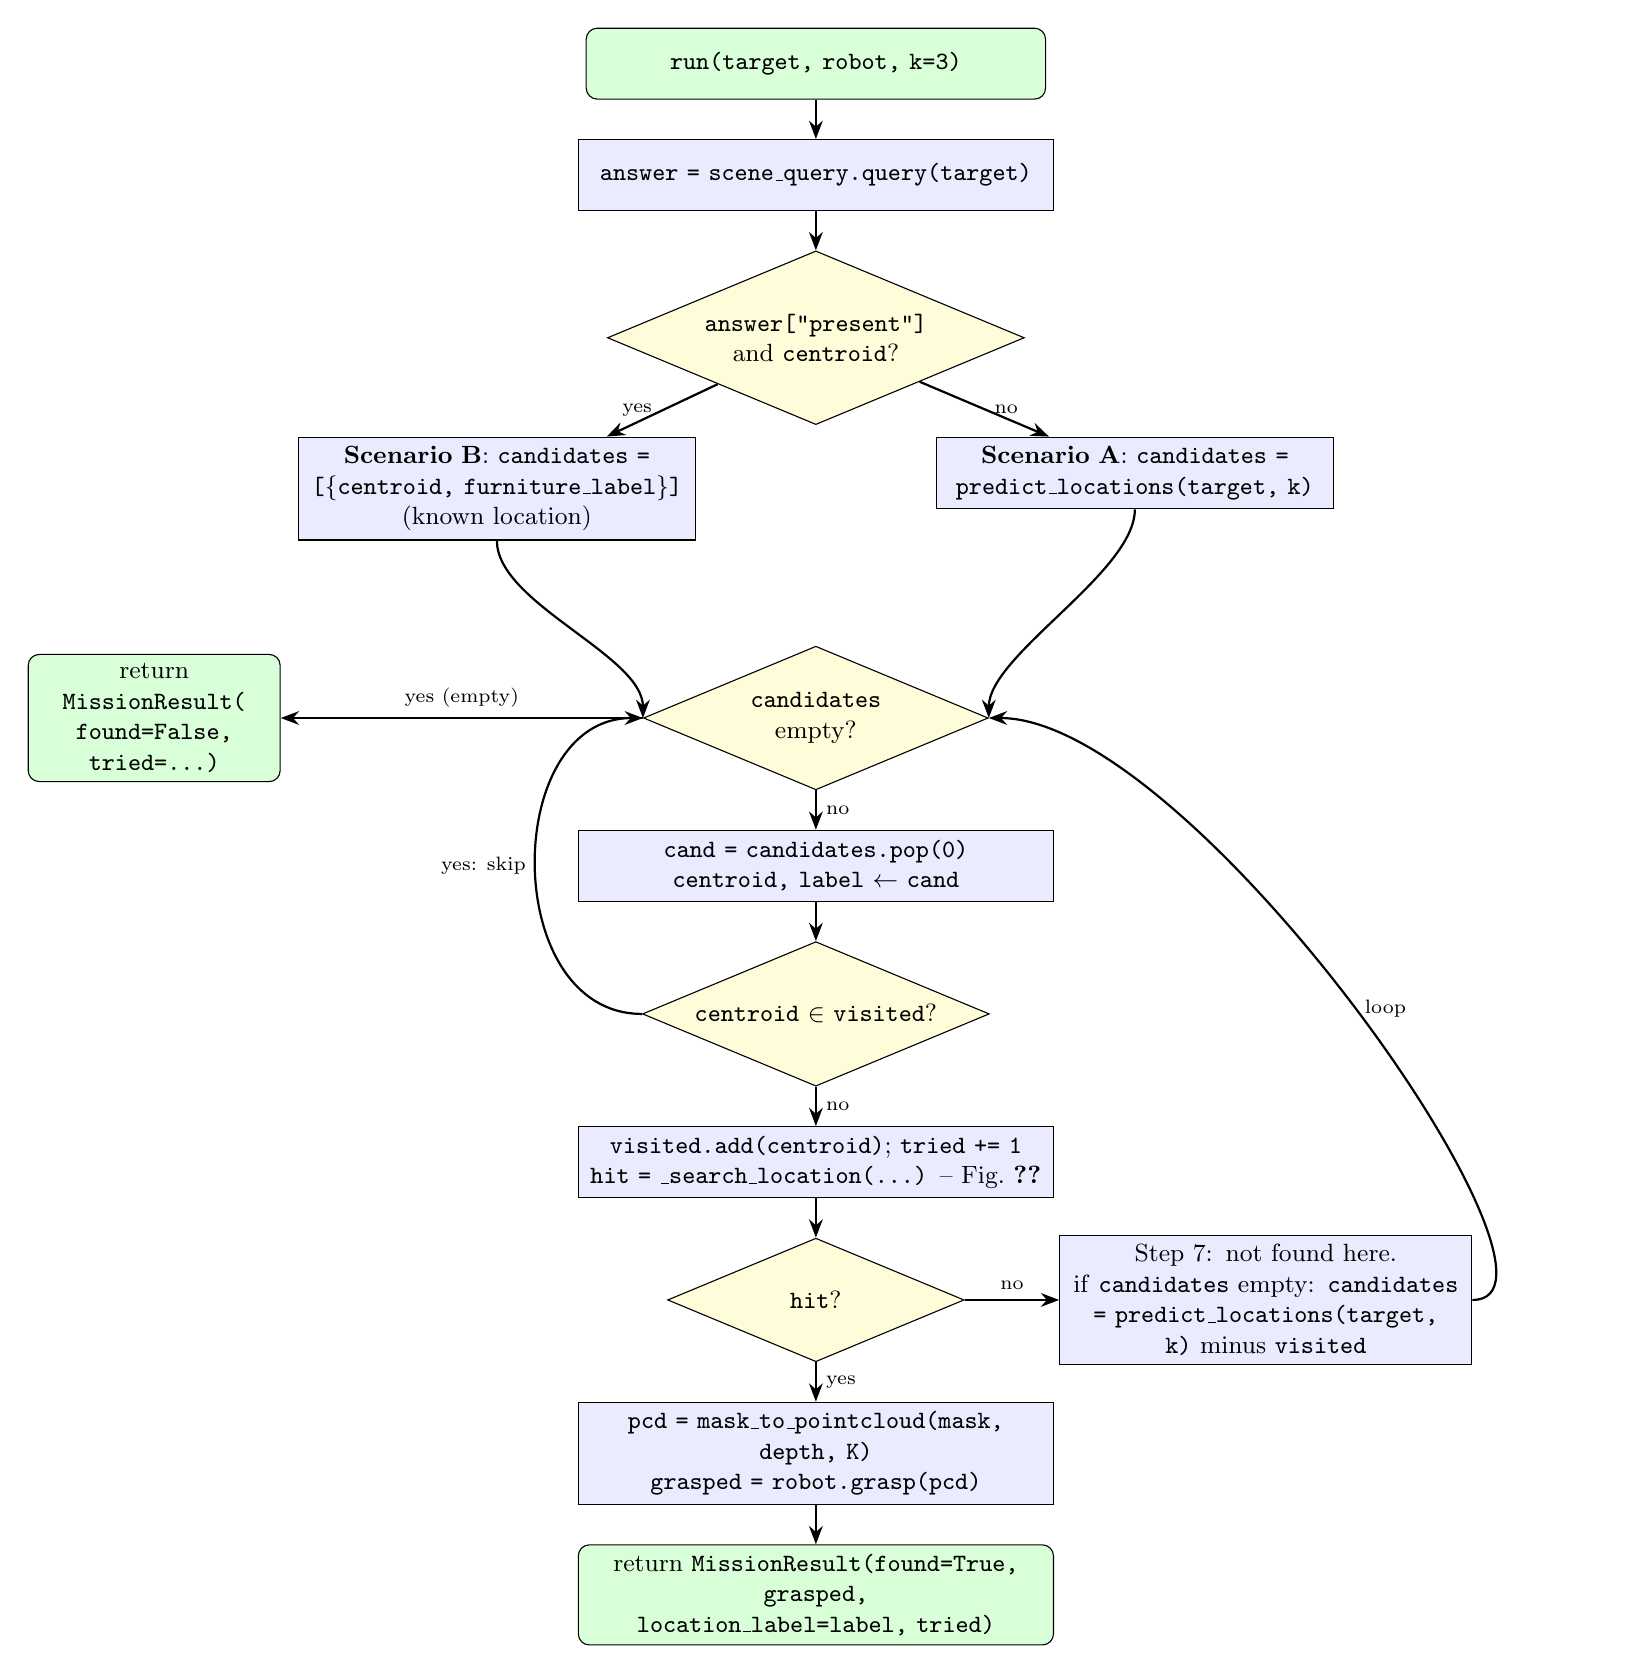
\begin{tikzpicture}[node distance=0.5cm]
\node[startstop, text width=5.6cm] (start) {\texttt{run(target, robot, k=3)}};
\node[process, below=of start, text width=5.8cm] (query) {\texttt{answer = scene\_query.query(target)}};
\node[decision, below=of query, text width=3.6cm] (scenario) {\texttt{answer["present"]} and \texttt{centroid}?};
\node[process, below left=0.7cm and 0.2cm of scenario, text width=4.8cm] (candB) {\textbf{Scenario B}: \texttt{candidates = [\{centroid, furniture\_label\}]} (known location)};
\node[process, below right=0.7cm and 0.2cm of scenario, text width=4.8cm] (candA) {\textbf{Scenario A}: \texttt{candidates = predict\_locations(target, k)}};
\node[decision, below=2.8cm of scenario, text width=2.6cm] (loopt) {\texttt{candidates} empty?};
\node[startstop, left=4.6cm of loopt, text width=2.6cm] (endnf) {return\\ \texttt{MissionResult(}\\ \texttt{found=False,}\\ \texttt{tried=...)}};
\node[process, below=of loopt, text width=5.8cm] (pop) {\texttt{cand = candidates.pop(0)}\\ \texttt{centroid, label} $\gets$ \texttt{cand}};
\node[decision, below=of pop, text width=3.6cm] (vis) {\texttt{centroid} $\in$ \texttt{visited}?};
\node[process, below=of vis, text width=5.8cm] (search) {\texttt{visited.add(centroid)}; \texttt{tried += 1}\\ \texttt{hit = \_search\_location(...)} -- Fig.~\ref{fig:searchloop}};
\node[decision, below=of search, text width=3cm] (hitc) {\texttt{hit}?};
\node[process, right=1.2cm of hitc, text width=5cm] (notfound) {Step 7: not found here.\\ if \texttt{candidates} empty: \texttt{candidates = predict\_locations(target, k)} minus \texttt{visited}};
\node[process, below=of hitc, text width=5.8cm] (graspn) {\texttt{pcd = mask\_to\_pointcloud(mask, depth, K)}\\ \texttt{grasped = robot.grasp(pcd)}};
\node[startstop, below=of graspn, text width=5.8cm] (endf) {return \texttt{MissionResult(found=True, grasped, location\_label=label, tried)}};

\draw[arrowline] (start) -- (query);
\draw[arrowline] (query) -- (scenario);
\draw[arrowline] (scenario) -- node[left, font=\scriptsize] {yes} (candB);
\draw[arrowline] (scenario) -- node[right, font=\scriptsize] {no} (candA);
\draw[arrowline] (candB.south) .. controls +(down:0.8cm) and +(up:0.8cm) .. (loopt.west);
\draw[arrowline] (candA.south) .. controls +(down:0.8cm) and +(up:0.8cm) .. (loopt.east);
\draw[arrowline] (loopt) -- node[above, font=\scriptsize] {yes (empty)} (endnf);
\draw[arrowline] (loopt) -- node[right, font=\scriptsize] {no} (pop);
\draw[arrowline] (pop) -- (vis);
\draw[arrowline] (vis) -- node[right, font=\scriptsize] {no} (search);
\draw[arrowline] (vis.west) .. controls +(left:1.8cm) and +(left:1.8cm) .. (loopt.west) node[midway, left, font=\scriptsize] {yes: skip};
\draw[arrowline] (search) -- (hitc);
\draw[arrowline] (hitc) -- node[above, font=\scriptsize] {no} (notfound);
\draw[arrowline] (hitc) -- node[right, font=\scriptsize] {yes} (graspn);
\draw[arrowline] (graspn) -- (endf);
\draw[arrowline] (notfound.east) .. controls +(right:1.6cm) and +(right:2.6cm) .. (loopt.east) node[midway, right, font=\scriptsize] {loop};
\end{tikzpicture}}
\caption{\texttt{search\_and\_fetch.run()}: scenario selection, the
candidate/visited loop, and the LLM fallback once the queue is empty. The
``\texttt{\_search\_location}'' box is expanded in Figure~\ref{fig:searchloop}.}
\label{fig:missionouter}
\end{figure}

\begin{figure}[H]
\centering
\resizebox{\textwidth}{!}{%
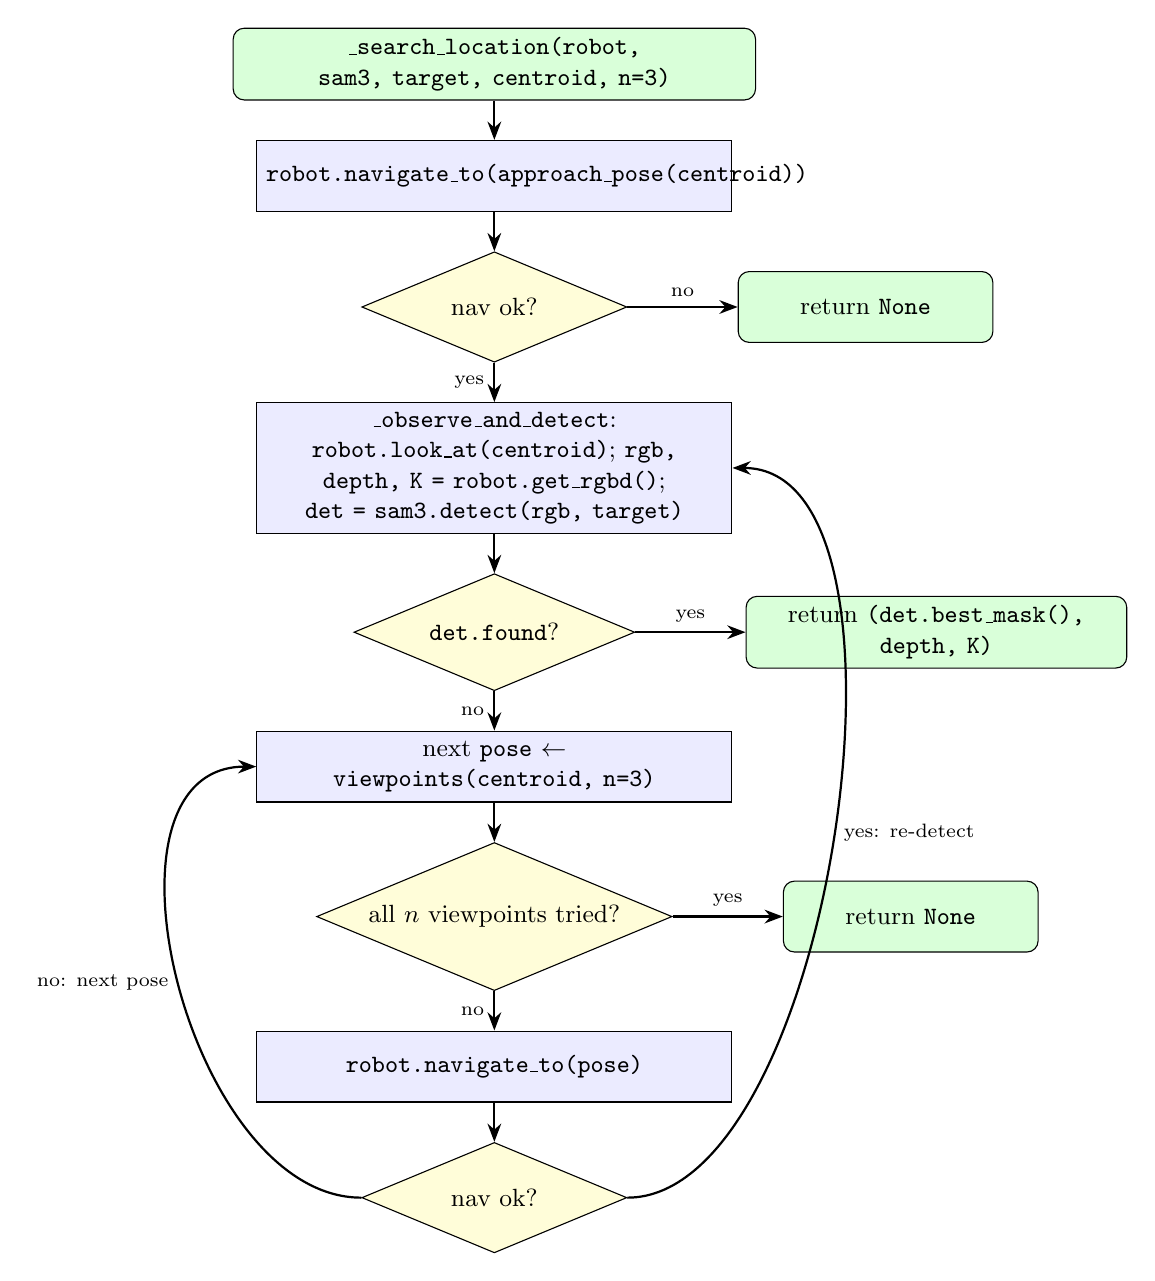
\begin{tikzpicture}[node distance=0.5cm]
\node[startstop, text width=6.4cm] (start) {\texttt{\_search\_location(robot, sam3, target, centroid, n=3)}};
\node[process, below=of start, text width=5.8cm] (navapp) {\texttt{robot.navigate\_to(approach\_pose(centroid))}};
\node[decision, below=of navapp, text width=2.6cm] (navok) {nav ok?};
\node[startstop, right=1.4cm of navok, text width=3cm] (retnone1) {return \texttt{None}};
\node[process, below=of navok, text width=5.8cm] (observe) {\texttt{\_observe\_and\_detect}:\\ \texttt{robot.look\_at(centroid)}; \texttt{rgb, depth, K = robot.get\_rgbd()}; \texttt{det = sam3.detect(rgb, target)}};
\node[decision, below=of observe, text width=2.8cm] (found) {\texttt{det.found}?};
\node[startstop, right=1.4cm of found, text width=4.6cm] (rethit) {return \texttt{(det.best\_mask(), depth, K)}};
\node[process, below=of found, text width=5.8cm] (vploop) {next \texttt{pose} $\gets$ \texttt{viewpoints(centroid, n=3)}};
\node[decision, below=of vploop, text width=3.6cm] (exhausted) {all $n$ viewpoints tried?};
\node[startstop, right=1.4cm of exhausted, text width=3cm] (retnone2) {return \texttt{None}};
\node[process, below=of exhausted, text width=5.8cm] (navvp) {\texttt{robot.navigate\_to(pose)}};
\node[decision, below=of navvp, text width=2.6cm] (navvpok) {nav ok?};

\draw[arrowline] (start) -- (navapp);
\draw[arrowline] (navapp) -- (navok);
\draw[arrowline] (navok) -- node[above, font=\scriptsize] {no} (retnone1);
\draw[arrowline] (navok) -- node[left, font=\scriptsize] {yes} (observe);
\draw[arrowline] (observe) -- (found);
\draw[arrowline] (found) -- node[above, font=\scriptsize] {yes} (rethit);
\draw[arrowline] (found) -- node[left, font=\scriptsize] {no} (vploop);
\draw[arrowline] (vploop) -- (exhausted);
\draw[arrowline] (exhausted) -- node[above, font=\scriptsize] {yes} (retnone2);
\draw[arrowline] (exhausted) -- node[left, font=\scriptsize] {no} (navvp);
\draw[arrowline] (navvp) -- (navvpok);
\draw[arrowline] (navvpok.west) .. controls +(left:2.2cm) and +(left:2.2cm) .. (vploop.west) node[midway, left, font=\scriptsize] {no: next pose};
\draw[arrowline] (navvpok.east) .. controls +(right:2.6cm) and +(right:2.6cm) .. (observe.east) node[midway, right, font=\scriptsize] {yes: re-detect};
\end{tikzpicture}}
\caption{\texttt{\_search\_location()} / \texttt{\_observe\_and\_detect()}: the
per-location active-perception loop (requirements 5, 7 and 8). The robot
first checks the direct approach pose, then orbits the target through up to
\texttt{n\_viewpoints} poses from \texttt{active\_perception.viewpoints()},
re-running detection from each one, before giving up on this location.}
\label{fig:searchloop}
\end{figure}

\section{Running the Pipeline}
\label{sec:run}

This section collects the commands used to run the whole system end to end,
in the order they are normally executed. All commands run inside the
devcontainer unless marked \emph{(host)}.

\subsection{One-time setup}

\begin{lstlisting}[style=sh,caption={Mask3D setup (host, only needed for requirement~9)}]
bash docker/mask3d/setup_mask3d.sh
\end{lstlisting}

\subsection{Bring up the simulation}

\begin{lstlisting}[style=sh,caption={Gazebo + Nav2 (Section~\ref{sec:architecture})}]
ros2 launch hsrb_gazebo_launch hsrc_apartment_world.launch.py
ros2 launch hsrb_rosnav_config navigation_launch.py map:=/home/ws/map.yaml
\end{lstlisting}

\begin{lstlisting}[style=sh,caption={SAM3 detection server (host, requirement~5)}]
export HF_TOKEN=hf_xxx   # accept the facebook/sam3 license on Hugging Face first
bash docker/sam3/run_sam3.sh
\end{lstlisting}

\begin{lstlisting}[style=sh,caption={IK solver (requirement~6)}]
ros2 launch fetcher ik_solver.launch.py
\end{lstlisting}

\subsection{Build the scene graph and room clusters (once per scene)}

\begin{lstlisting}[style=sh,caption={Requirement~1: scene graph from Gazebo ground truth (Section~\ref{sec:scenegraph})}]
ros2 run fetcher gazebo_scene_graph
# or, equivalently, without ROS:
python -m core.perception.scene_graph.build_scene_graph_gazebo [--visualize]
\end{lstlisting}

\begin{lstlisting}[style=sh,caption={Requirement~9: scene graph from a real RGB-D scan (Section~\ref{sec:mask3d})}]
bash docker/mask3d/run_mask3d.sh [workspace] [mask3d_repo]   # host
python -m core.perception.scene_graph.build_scene_graph [--workspace <path>] [--visualize]
\end{lstlisting}

\begin{lstlisting}[style=sh,caption={Requirement~2: room clustering (Section~\ref{sec:rooms})}]
DEEPSEEK_API_KEY=<key> python -m core.llm_zone.room_clustering
\end{lstlisting}

\subsection{Run the mission (requirements 3--7, single command)}

\begin{lstlisting}[style=sh,caption={Requirement~10: single-command search and fetch (Section~\ref{sec:singlecmd})}]
DEEPSEEK_API_KEY=<key> ros2 run fetcher search_and_fetch "<object>"
\end{lstlisting}

For ad-hoc testing of just the scene-reasoning layer (no robot), the
DeepSeek-backed query can be run standalone:

\begin{lstlisting}[style=sh,caption={Scene query only (Section~\ref{sec:scenario})}]
DEEPSEEK_API_KEY=<key> python core/llm_zone/scene_query.py "something to drink"
\end{lstlisting}

\section{Conclusion}

Every demo-day requirement maps to a small, single-purpose module: Gazebo's
own SDF files drive scene-graph geometry (\S\ref{sec:scenegraph}), DeepSeek
clusters rooms and resolves search targets (\S\ref{sec:rooms},
\S\ref{sec:scenario}), and the navigate/observe/grasp loop
(Figures~\ref{fig:missionouter}--\ref{fig:searchloop}) is shared verbatim
between Scenario A and Scenario B. The same \texttt{SceneGraph} /
\texttt{ObjectNode} representation, and the same JSON files, are produced
whether the source is Gazebo's ground truth (\S\ref{sec:worldparse}--\S\ref{sec:results})
or a real Mask3D scan (\S\ref{sec:mask3d}), so the LLM and mission layers are
unaware of which one was used. Most importantly for this report's original
motivation: nothing in \S\ref{sec:scenegraph} is hand-picked -- every object's
position comes from \texttt{apartment.world.xacro}'s \texttt{<include><pose>},
and every object's size and shape comes from parsing that same object's own
\texttt{model.sdf} collision geometry (\S\ref{sec:geomextract}), so adding,
moving, or resizing an object in Gazebo automatically and correctly updates
the scene graph with no code changes.

\end{document}
